\documentclass[a4paper,12pt]{article}
%All Layout Packages are defined in the Header.tex
\usepackage[utf8]{inputenc}
\usepackage[english]{babel}
\usepackage{fancyhdr}

%This is to print solutions or not
\usepackage{ifthen}

%This is to include src code
\usepackage{listings}
\lstset{ %
  backgroundcolor=\color{white},   % choose the background color; you must add \usepackage{color} or \usepackage{xcolor}
  basicstyle=\footnotesize,        % the size of the fonts that are used for the code
  breakatwhitespace=false,         % sets if automatic breaks should only happen at whitespace
  breaklines=true,                 % sets automatic line breaking
  captionpos=b,                    % sets the caption-position to bottom
  commentstyle=\color{commentsColor}\textit,    % comment style
  deletekeywords={...},            % if you want to delete keywords from the given language
  escapeinside={\%*}{*)},          % if you want to add LaTeX within your code
  extendedchars=true,              % lets you use non-ASCII characters; for 8-bits encodings only, does not work with UTF-8
  frame=tb,	                   	   % adds a frame around the code
  keepspaces=true,                 % keeps spaces in text, useful for keeping indentation of code (possibly needs columns=flexible)
  keywordstyle=\color{keywordsColor}\bfseries,       % keyword style
  language=Python,                 % the language of the code (can be overrided per snippet)
  otherkeywords={*,...},           % if you want to add more keywords to the set
  numbers=left,                    % where to put the line-numbers; possible values are (none, left, right)
  numbersep=5pt,                   % how far the line-numbers are from the code
  numberstyle=\tiny\color{commentsColor}, % the style that is used for the line-numbers
  rulecolor=\color{black},         % if not set, the frame-color may be changed on line-breaks within not-black text (e.g. comments (green here))
  showspaces=false,                % show spaces everywhere adding particular underscores; it overrides 'showstringspaces'
  showstringspaces=false,          % underline spaces within strings only
  showtabs=false,                  % show tabs within strings adding particular underscores
  stepnumber=1,                    % the step between two line-numbers. If it's 1, each line will be numbered
  stringstyle=\color{stringColor}, % string literal style
  tabsize=2,	                   % sets default tabsize to 2 spaces
  title=\lstname,                  % show the filename of files included with \lstinputlisting; also try caption instead of title
  columns=fixed                    % Using fixed column width (for e.g. nice alignment)
}


%Use this to customize margins
\usepackage[
  top=2cm,
  bottom=2cm,
  left=1cm,
  right=1cm,
  headheight=17pt, % as per the warning by fancyhdr
  includehead,includefoot,
  heightrounded, % to avoid spurious underfull messages
]{geometry} 

%Use this to customize headers
\pagestyle{fancy}
\fancyhf{}
\fancyhead[LE,RO]{Version: \today}
\fancyhead[RE,LO]{Geophysics Exercises}
\fancyfoot[CE,CO]{\leftmark}
\fancyfoot[LE,RO]{\thepage}
\usepackage{graphicx}
\renewcommand{\headrulewidth}{2pt}
\renewcommand{\footrulewidth}{1pt}


%Use this to customize tables
\usepackage[table]{xcolor}
\usepackage{tabularx}
\usepackage{booktabs}


\setlength{\arrayrulewidth}{1mm}
\setlength{\tabcolsep}{18pt}
\renewcommand{\arraystretch}{1.5}


%Use this to customize colors
\definecolor{myblue}{rgb}{0.0, 0.53, 0.74}
\definecolor{myred}{rgb}{1.0, 0.8, 0.89}
\definecolor{babyblueeyes}{rgb}{0.63, 0.79, 0.95}
\definecolor{beaublue}{rgb}{0.74, 0.83, 0.9}
\definecolor{bluegray}{rgb}{0.4, 0.6, 0.8}
\definecolor{commentsColor}{rgb}{0.497495, 0.497587, 0.497464}
\definecolor{keywordsColor}{rgb}{0.000000, 0.000000, 0.635294}
\definecolor{stringColor}{rgb}{0.558215, 0.000000, 0.135316}
\definecolor{burgundy}{rgb}{0.5, 0.0, 0.13}
%Here some pre-defined commands
\newcommand{\ProtocolTable}[6]
{
\begin{table}[]
\begin{tabular}{|p{1.8cm} p{3.8cm} p{1.8cm} p{2.0cm}|}
\hline
 \rowcolor{beaublue}\textbf{Name}:&\multicolumn{3}{l}{#1} \\
 \rowcolor{beaublue}\textbf{Folder:}&\multicolumn{3}{l}{#2} \\
 \rowcolor{beaublue}\textbf{Instrument:}&#3&\textbf{Date:}&#4 \\
  \rowcolor{beaublue}\textbf{Operator:}&#5&\textbf{Location:}&#6\\
\hline
\end{tabular}
\end{table}
}
\usepackage{enumitem}
\usepackage{blindtext}
\usepackage{afterpage}
\usepackage{lipsum,lmodern}
\usepackage[most]{tcolorbox}
\tcbuselibrary{skins}
\usepackage{hyperref}

%no indents at paragraphs 
\setlength\parindent{0pt}

%% Oh yes. TIKZ pictures / graphs
%% -------------------------------------
\usepackage{tikz}
\usepackage{pgfplots}
\usepackage{tikz-3dplot}
\usetikzlibrary{calc,fadings,decorations.pathreplacing,shadings,intersections}


\newif\ifanswers
\answerstrue % comment out to hide answers


\begin{document}
\newcounter{mycounter}
\begin{tcolorbox}[enhanced jigsaw,breakable,pad at break*=1mm,
    colback=blue!5!white,colframe=burgundy,title=Expectations for Exercises]
    Exercises are an important part of the Geophysics lecture. They will treat some aspects of the lecture in more detail, but also cover new ground. We expect that you work on the exercises at home and we will discuss questions and solutions interactively together. Questions that are marked with 'Extra' are not required but geared to stir
     your further interest. We will surely support you if you tackle those as well. 
\end{tcolorbox}

% \section{Exercises for Gravity Method 1}
% \textbf{Version:} \today 

% \textbf{Context:} Videos Introduction \& Gravity 01, Gravity 02

% \textbf{Timing:} All gravity exercises should be completed by week 3.

%   \subsection{Detection of a spherical object in the sub-surface}
\label{Sec:SphereInSubsurface}
\begin{enumerate}[label=(\alph*)]
  \item Consider a spherical object with radius $R$ located at depth $z$ below the surface, and a gravimeter that is moved along the surface across the anomaly (Fig.\ref{Fig:SphereInSubsurface}). Derive an analytical expression for the expected \textit{vertical} anomaly $g_z$ as a function of the lateral distance $x$ and depth $z$. Calculate the maximum anomalies that you would expect for some realistic settings (e.g., a limestone cave). Only consider the anomaly relative to a reference point far away from the target and not the total gravitational field.

  \item Use a piece of paper or a software of your choice (e.g., Excel, SciDAVis, Matlab, Python) and visualize the expected vertical gravity anomaly for a specific setting as a function of lateral distance $x$. Show how this profile changes as you vary the depth of the object. 

  \item Sometimes results in the gravity method are expressed in \textit{mGal} with 1 Gal = 0.01 m s$^{-2}$. Transfer your results to those units and post a picture of your graph in the forum.

  \item We now investigate how we can estimate the depth of the object from an anomaly as derived in (a,b). For this you have to derive an expression that links the half-width of the anomaly (i.e. $g_z = \frac{1}{2}g_{z,max}$ for $x=x_{1/2}$) to the depth $z$ of the object. Derive this relationship which has the form $z = c x_{1/2}$. Why is such a relationship be useful?
\end{enumerate}

\begin{figure}
\centering
\begin{minipage}[c]{0.5\textwidth}
\begin{center}
    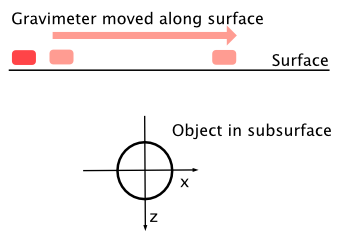
\includegraphics[width=\textwidth]{Figures/Gravimetry/Gravimetry01_SphereSketch.png}
\end{center}
\caption{Sketch for problem \ref{Sec:SphereInSubsurface}. It is easiest to choose a coordinate system with the origin inside the subsurface object.}
\label{Fig:SphereInSubsurface}
\end{minipage}
\end{figure}

\ifanswers
    \begin{tcolorbox}[enhanced jigsaw,breakable,pad at break*=1mm,
    colback=blue!5!white,colframe=babyblueeyes,title=Solutions]
     \begin{center}
       
\includegraphics[width=0.5\textwidth]{Figures/Gravimetry/Gravimetry01_SphereSketchSolutions.png}
    \end{center}
    \textbf{(a)} Because we have a spherical object, we can use the shell theorem and treat it as a point mass. The gravitational force exhibited by the sphere is:
    $$
    \vec{g} = -G\frac{M}{r^2}\hat{r}
    $$
    where $\hat{r}$ is the unit vector pointing from the center of mass to our gravimeter at the surface. The minus sign makes sure that the force is attractive (and not repulsive). The mass anomaly $M$ formulated in a relative sense of the sphere is given by:
    $$
    M = \frac{4}{3}\pi R^3 \Delta \rho
    $$
    At distance $x$ the distance to the sphere is $r=\sqrt{x^2+z^2}$. The gravimeter only measures the vertical component of $\vec{g}$:
    $$
    g_z = -|\vec{g}|\cos\phi = -|\vec{g}|\frac{z}{r}
    $$
  
    which brings us to:
    \begin{eqnarray*}
    g_z &=& -\frac{4}{3}\pi R^3 \Delta \rho \frac{G}{r^2} \frac{z}{r} \\
        &=& -\frac{4}{3}\pi R^3 \Delta \rho \frac{G}{r^3} z \\
        &=& -\frac{4}{3}\pi R^3 \Delta \rho G \frac{z}{(x^2+z^2)^\frac{3}{2}}
    \end{eqnarray*}
    We will encounter the maximum value of the anomaly at $x = 0$ (directly above the target):
    $$
    g_{z,max} = \frac{4}{3}\pi R^3 \Delta \rho G \frac{1}{z^2}
    $$
    which for the limestone cave example is approximately -0.35 mGal (see below).
    

    \textbf{(b, c)}
    \lstinputlisting[language=matlab]{../../Src/Exercises/Gravimetry/Gravimetry01_SphereVisualization.m}
    \begin{center}
        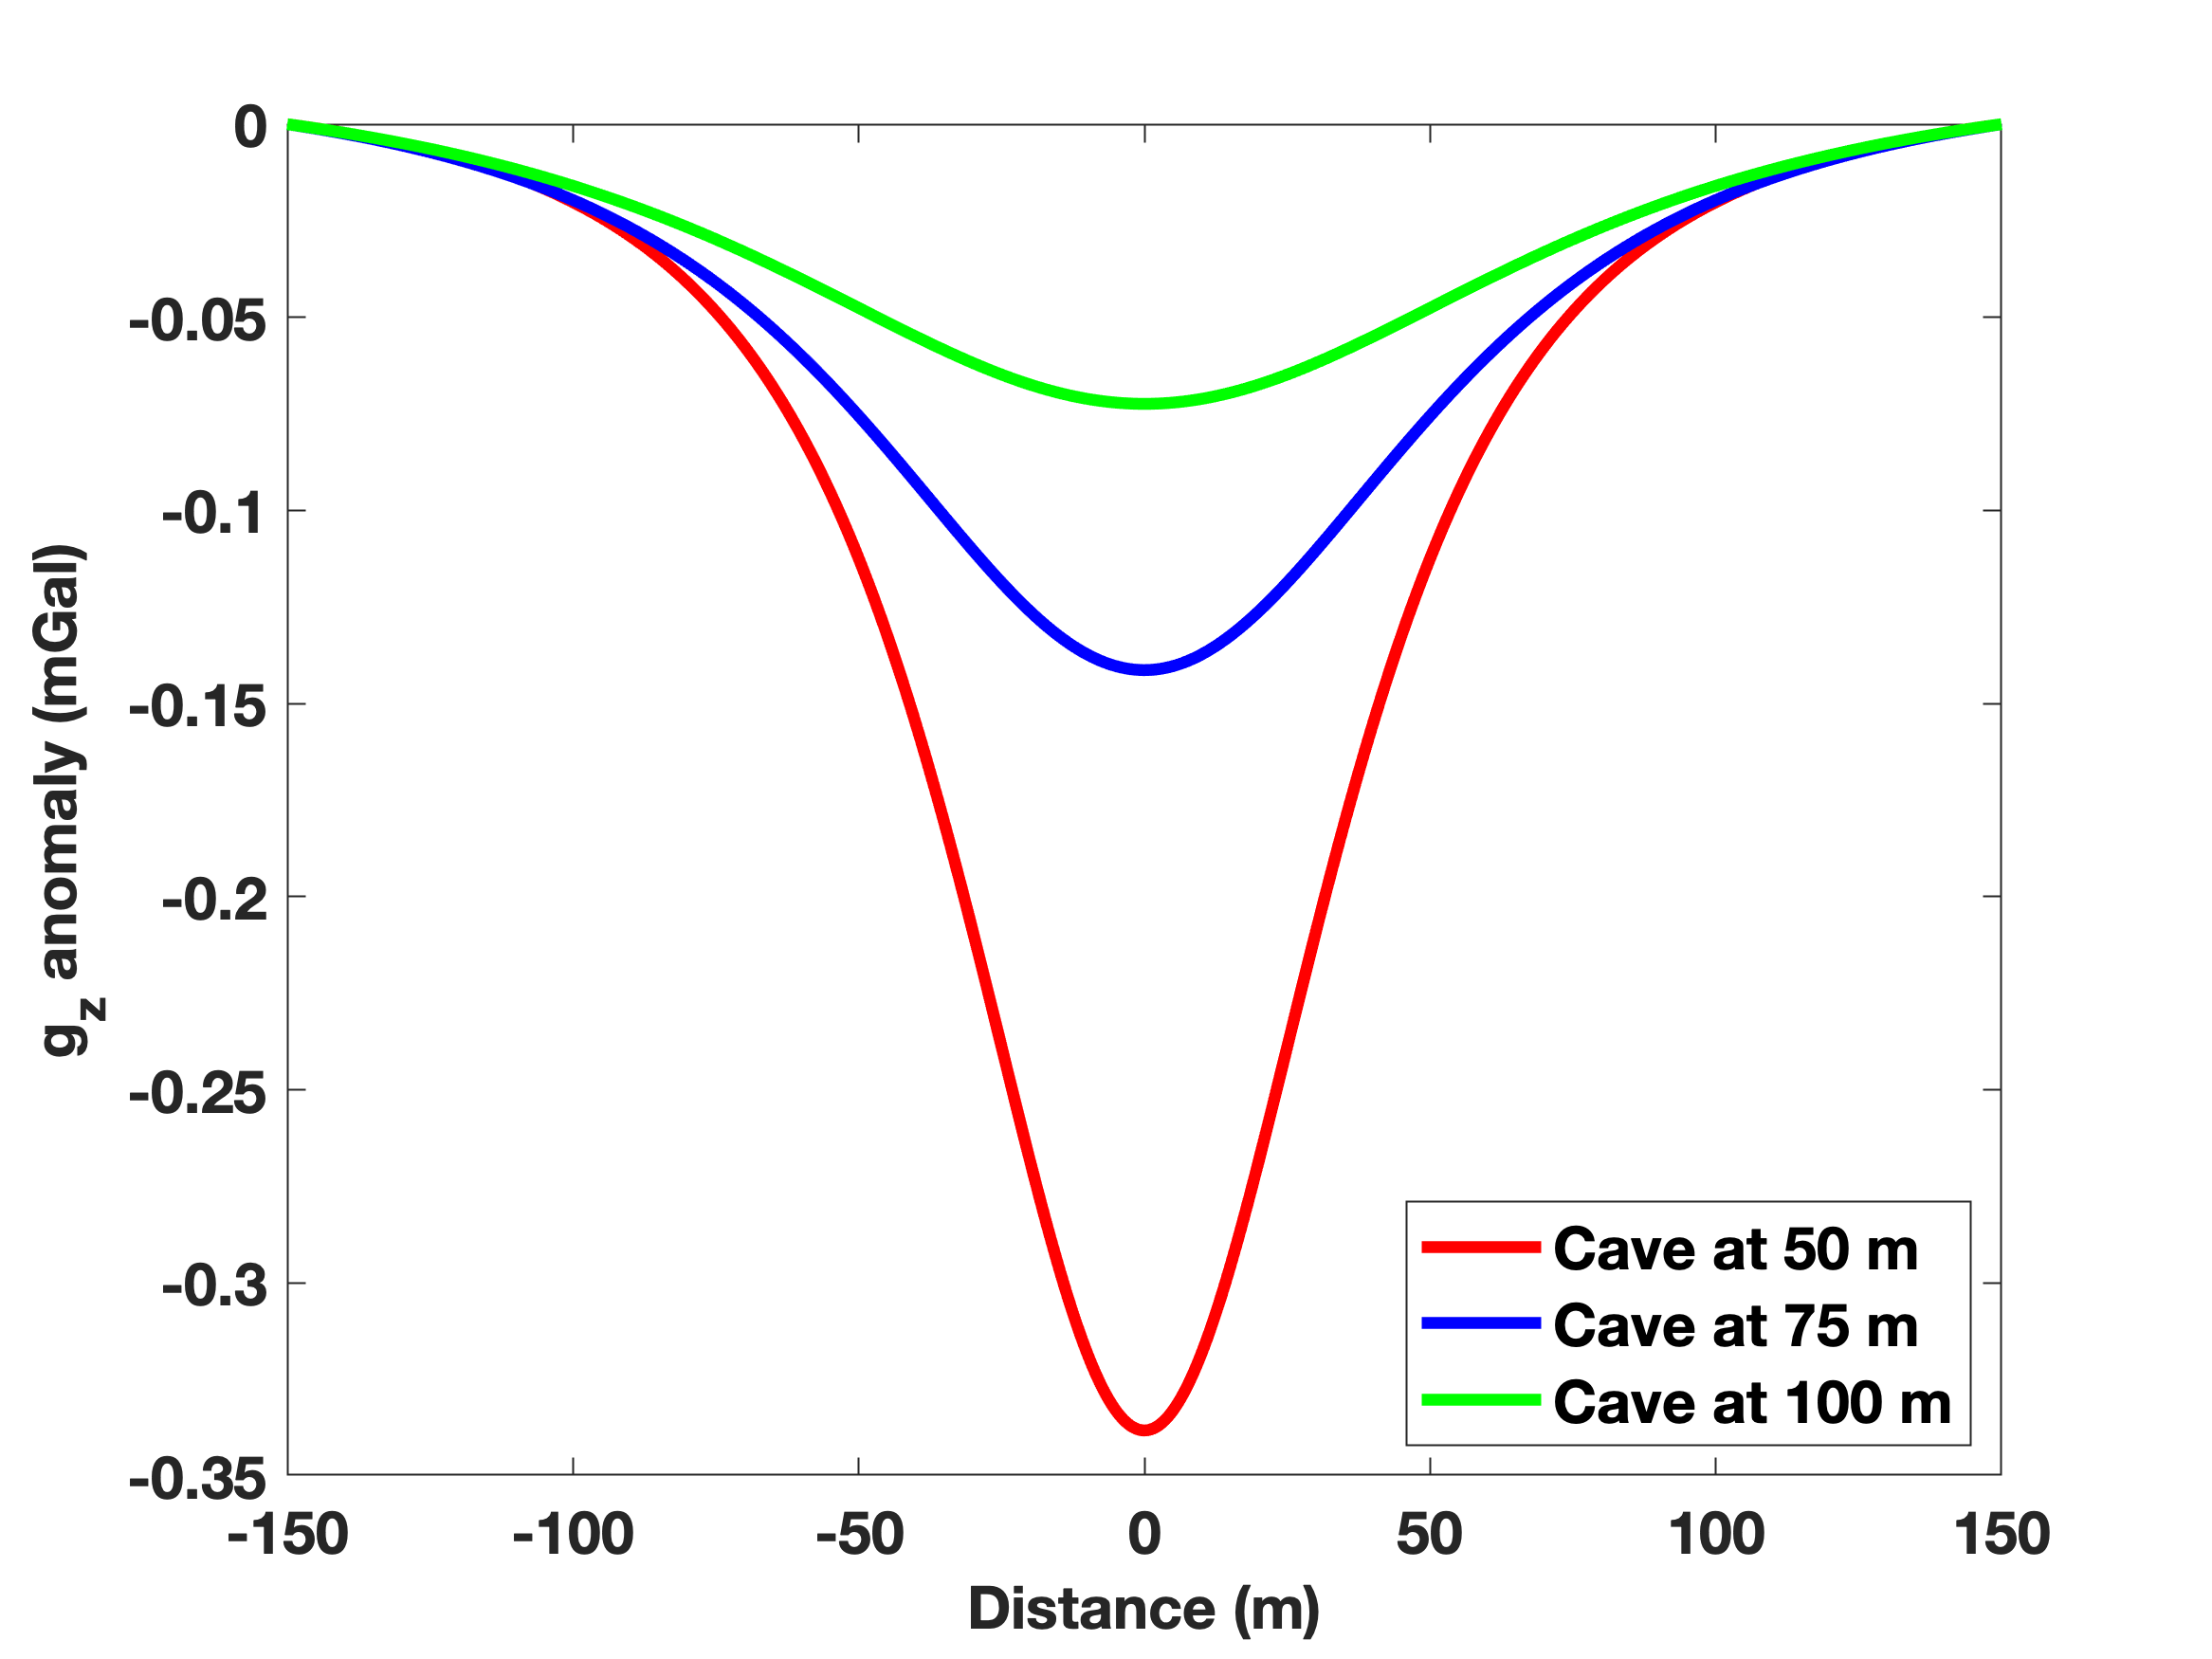
\includegraphics[width=0.5\textwidth]{Figures/Gravimetry/Gravimetry01_Visualization.png}
    \end{center}
 
    \textbf{(d)}This requires some arithmetic manipulation to isolate $z$.
\begin{eqnarray*}
g_z &=\frac{1}{2}g_{z,max} \\
\rightarrow \frac{z}{(x^2_{1/2}+z^2)^\frac{3}{2}} &= \frac{1}{2z^2}\\
\rightarrow \frac{z^3}{(x^2_{\frac{1}{2}}+z^2)^\frac{3}{2}}&= \frac{1}{2}\\
\rightarrow \frac{z^2}{(x^2_{\frac{1}{2}}+z^2)}&= \frac{1}{2^{2/3}}\\
\rightarrow \frac{1}{(\frac{x^2_{\frac{1}{2}}}{z^2}+1)}&= \frac{1}{2^{2/3}}\\
\rightarrow 1 = \frac{1}{2^{2/3}} (\frac{x^2}{z^2}+1)\\
\rightarrow z = \frac{x_{1/2}}{\sqrt{2^{\frac{2}{3}}-1}}\approx 1.305 x_{1/2}
\end{eqnarray*}
Those expressions can be useful to estimate the depth of an object from an observed anomaly without using a full forward model. However, this only works if the object is close to spherical (which we usually don't know necessarily ahead of time.) Similar estimates exists for other shapes (e.g., horizontal and vertical cylinders).
\end{tcolorbox}
\fi
%   \subsection{Gravitational acceleration inside the Earth}
Knowing the gravitational acceleration \textit{inside} the Earth is important, e.g., for understanding processes related to mantel convection.
\begin{enumerate}[label=(\alph*)]
  \item Use the consequences of the shell theorem to predict the gravitational acceleration $g(r)$ inside a spherical Earth. First assume that the Earth's density is constant, then that it decreases linearly with distance from the center. Assume that the density in the core is approximately $\rho_{core} = 13 \frac{g}{cm^3}$ and in the crust approximately $\rho_{crust} = 2.7 \frac{g}{cm^3}$.

  \item Draw the results on a x-y graph on paper or using a software of your choice.

  \item The PREM model (Fig. \ref{Fig:PREM})provides an observationally constrained estimate of the density distribution inside the Earth. Knowing the shape of this profile, what is your guess of the gravitational acceleration inside the Earth? Why is it more difficult for you to calculate this quantitatively compared to the previous cases of constant and linearly varying density?

  \item Extra: Calculate the gravitational acceleration inside the Earth based on the PREM model using Matlab/Python/Excel. The data can be found on Ilias.
\end{enumerate}

\begin{figure}
    \label{Fig:PREM}
    \begin{center}
    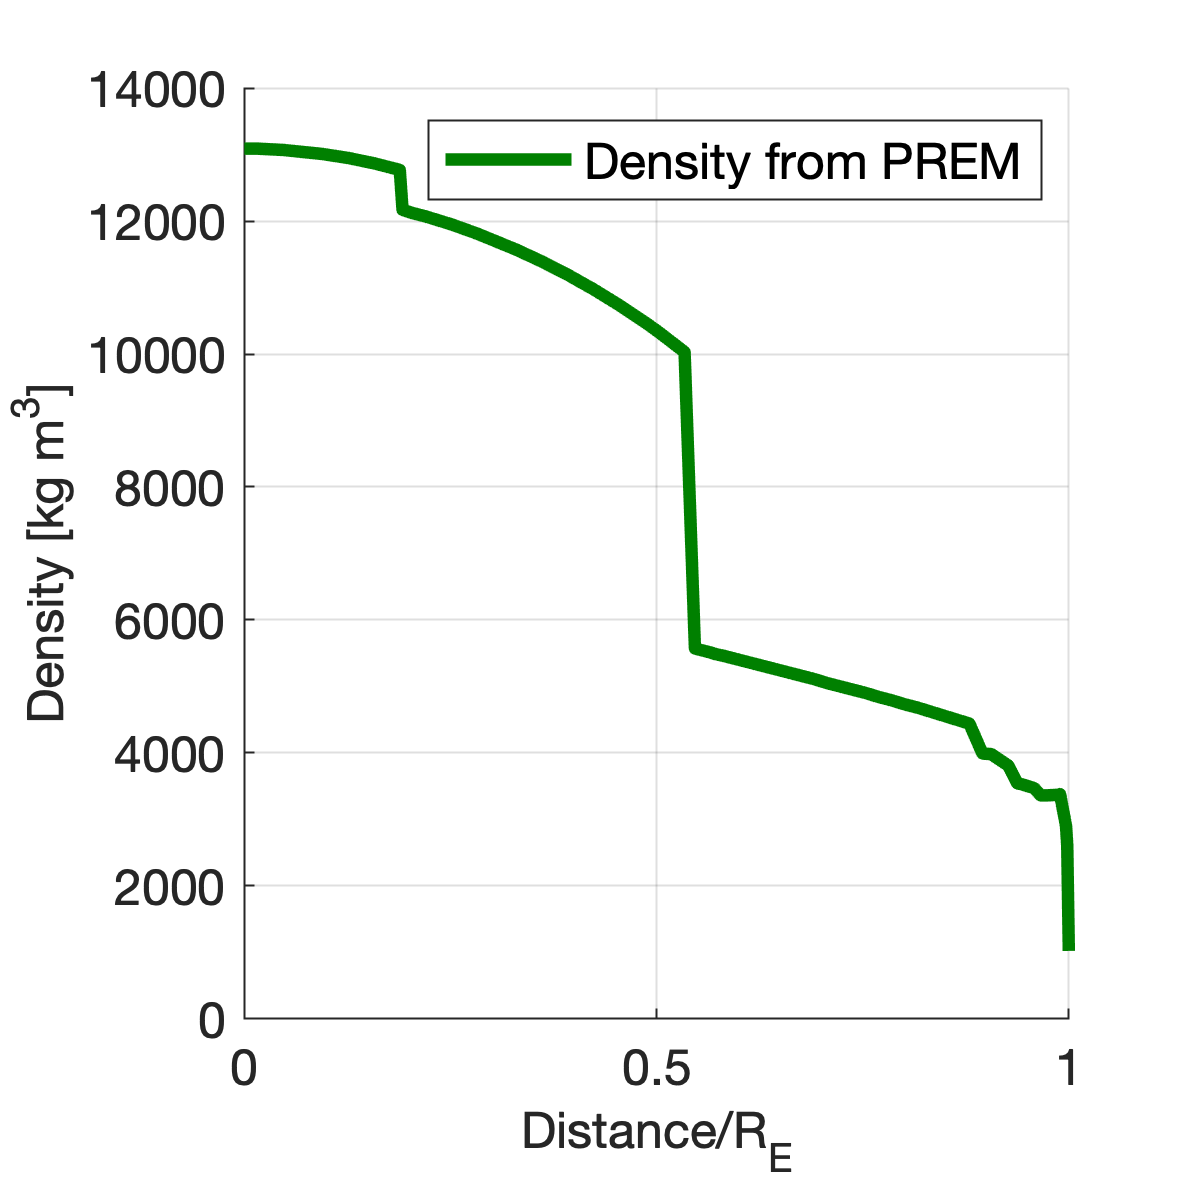
\includegraphics[width=0.5\textwidth]{Figures/Gravimetry/Gravimetry01_PREM.png}
    \caption{The Preliminary Reference Earth Mode (Dziewonski, A. M. \& Anderson, D. L, 1981).}
    \end{center}
\end{figure}
\ifanswers
    \begin{tcolorbox}[enhanced jigsaw,breakable,pad at break*=1mm,
    colback=blue!5!white,colframe=babyblueeyes,title=Solutions,
    watermark color=white]
 
      (a) At location $l<R$ inside the Earth, we do not need to worry about the mass distribution for distances $>l>R$ as these will cancel out due to the spherical symetry. Also the the acceleration will only have a radial component. Hence,
    \begin{equation}
        |\vec{g}(l)| = G\frac{M}{l^2}
    \end{equation}
    where $M$ is mass contained in the sphere with radius $l$. How does $M$ change as we change $l$? In this spherical symetry it is best to adopt spherical coordinates so that we can write: 
    \begin{eqnarray}
    M &=& \int \rho dV \\ 
    &=& \int_0^{\frac{\pi}{2}} d\theta \sin(\theta) \int_0^{2\pi}  d\phi \int_0^l dl\,\rho\,l^2 dV
    \end{eqnarray}
    this is a fairly complicated way of writing something that you know by heart (i.e. the density times the volume of a sphere), but this is a good oppertunity to make use of spherical coordinates. Most importantly, it is worthwhile to remember that the volume element $dV = l^2 \sin(\theta)drd\theta d\phi$ is quite different from the cartesian coordinates that you are used to otherwise. Also take a moment and understand why the integration limits are the way they are. Solving the integral step by step for the case of a constant density:
    \begin{eqnarray}
        M &=& \rho \int_0^{\frac{\pi}{2}} d\theta \sin(\theta)\int_0^{2\pi}  d\phi \int_0^l l^2 dl \\
         &=&\rho 2\pi \int_0^{\frac{\pi}{2}} d\theta \sin(\theta)\int_0^l l^2dl\\
         &=&\rho 4\pi \int_0^l l^2dl \\ 
         &=&\rho \frac{4}{3}\pi l^3
    \end{eqnarray}
    Plugging (7) into (1) then results for $l<R$:
    \begin{equation}
        |\vec{g}(l)| = G  \rho \frac{4}{3}\pi \frac{l^3}{l^2} = G  \rho \frac{4}{3}\pi l
    \end{equation}
    so the gravitational acceleration increases linearly with distance from the Earth's center as long as $l<R$ and $\rho$ is constant. A linear decrease of density with increasing distance can be parameterized as:
    \begin{equation}
        \rho(l) = \frac{\rho_{crust}-\rho_{core}}{R} (l-R) + \rho_{crust} = \frac{\rho_{crust} - \rho_{core}}{R}l+\rho_{core}
    \end{equation}
    As the density now changes with $l$ we cannot take it out of the integration. In particular for eq. (6) this means:
    \begin{eqnarray}
        M &=& 4\pi \int_0^l dl \left(\frac{\rho_{crust} - \rho_{core}}{R}l^3+\rho_{core}l^2\right)\\
          &=& 4\pi \left(\frac{\rho_{crust} - \rho_{core}}{4R}l^4+\frac{1}{3}\rho_{core}l^3 \right)
    \end{eqnarray}
    so that:
    \begin{eqnarray}
        |\vec{g}(l)| &=& 4 G \pi \frac{1}{l^2} \left(\frac{\rho_{crust} - \rho_{core}}{4R}l^4+\frac{1}{3}\rho_{core}l^3 \right) \\
        &=& 4 G \pi \left(\frac{\rho_{crust} - \rho_{core}}{4R}l^2+\frac{1}{3}\rho_{core}l \right)
    \end{eqnarray}
    \begin{center}
        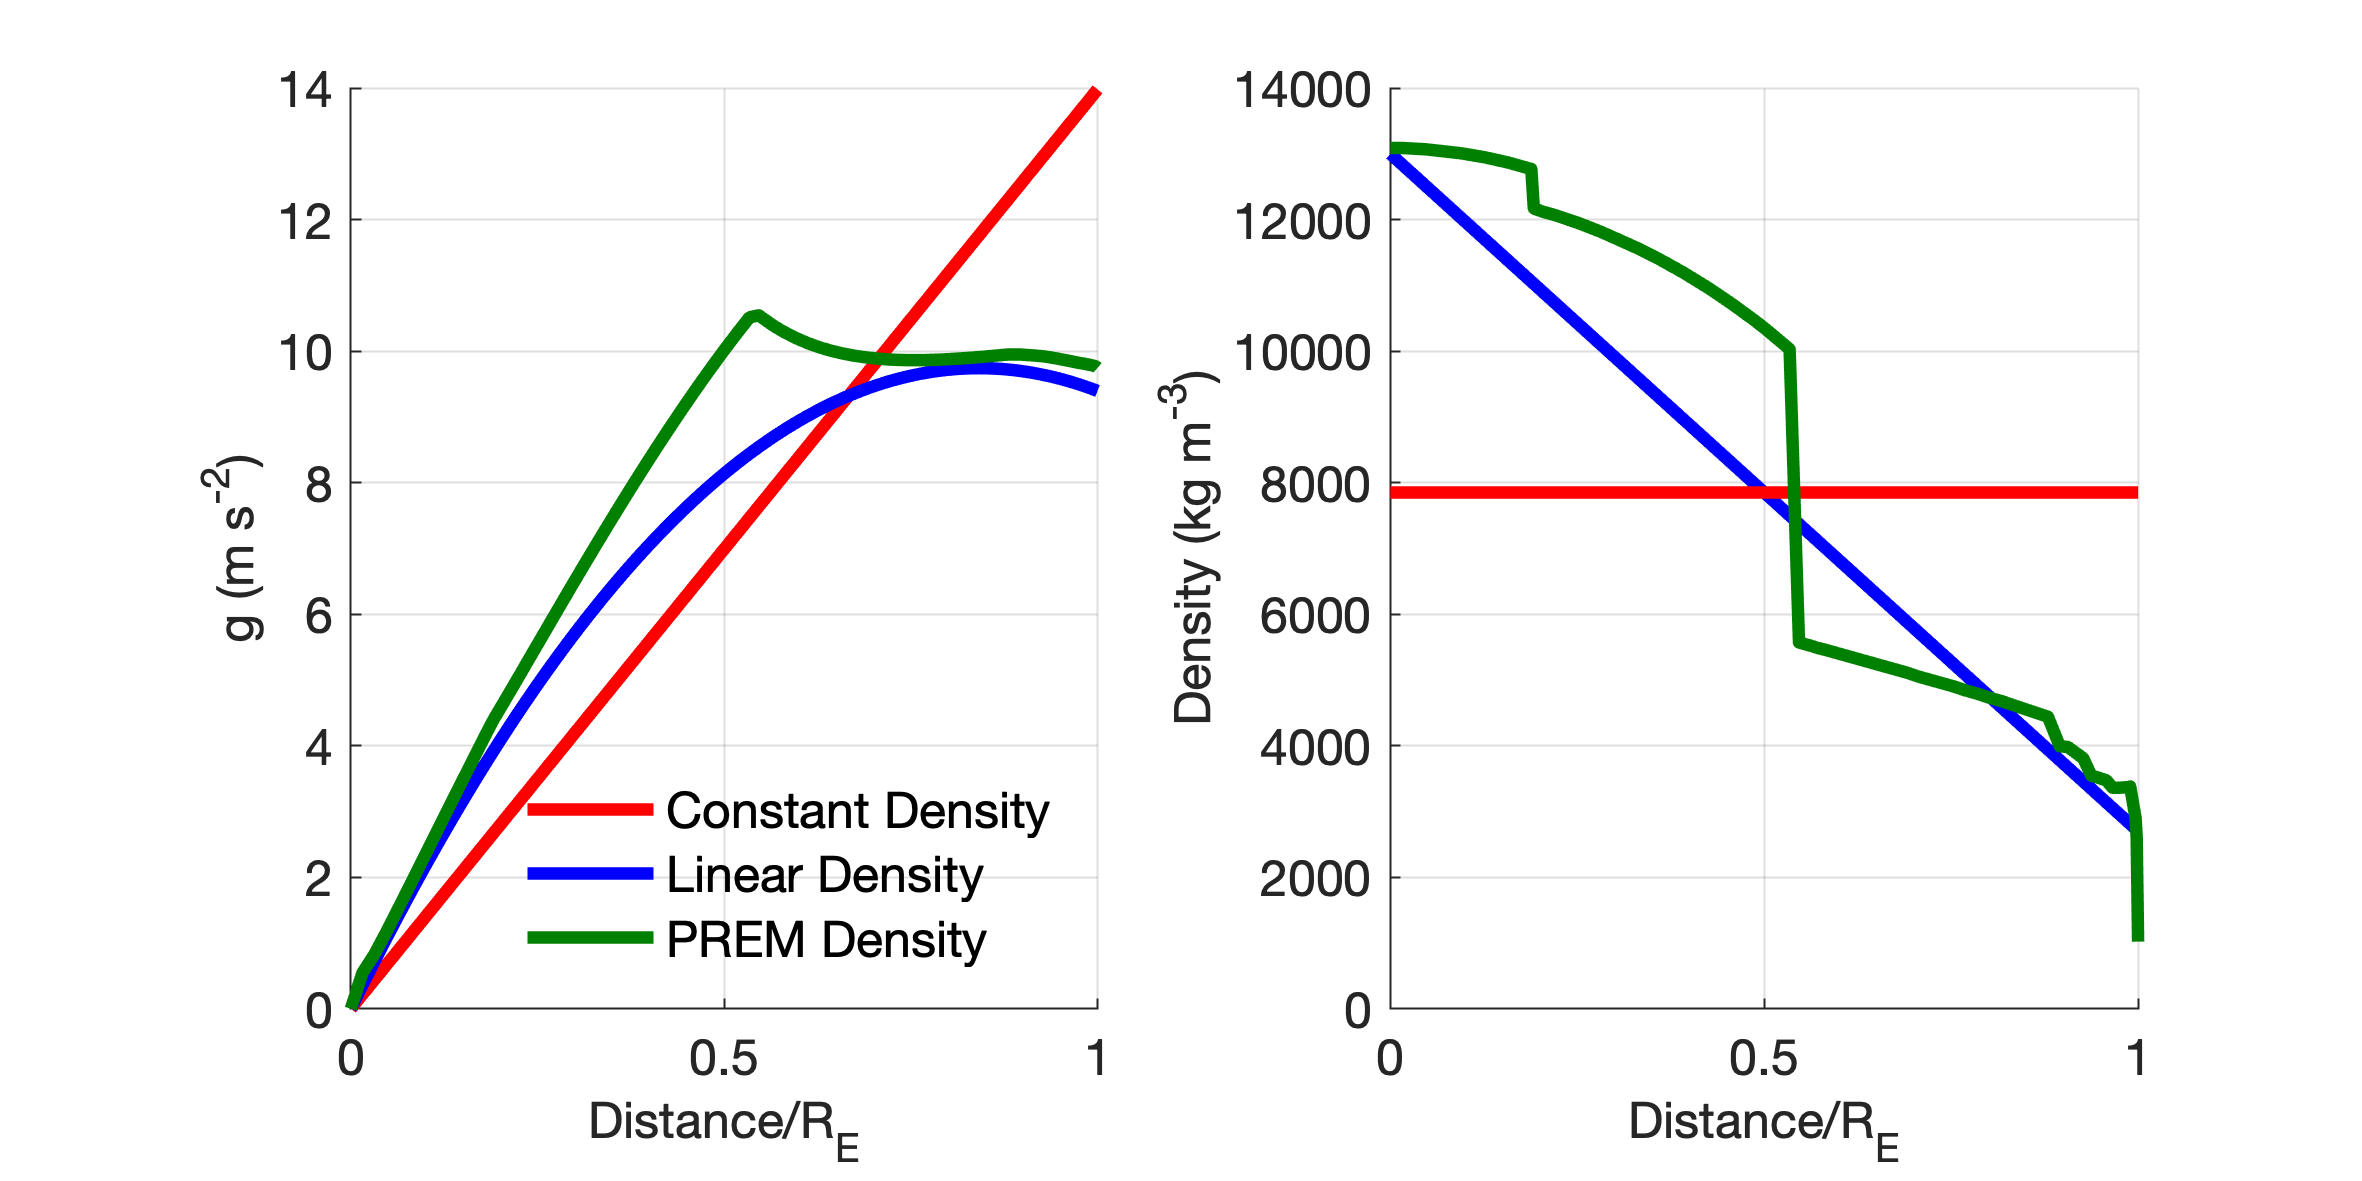
\includegraphics[width=0.99\textwidth]{Figures/Gravimetry/Gravimetry01_GravityInsideEarth.png}
     \end{center}
     so that the gravitational acceleration now changes quadratically as shown in the Figure above. Is this realistic? We will have to compare it with a realistic dataset such as the PREM model.

  (c) Because we don't have an analytical expression for the PREM density model, we cannot pursue an analytical integration as done in the previous two cases. Hence we do it numerically:
     \lstinputlisting[language=matlab]{../../Src/Exercises/Gravimetry/Gravimetry03_GravityInsideSphere.m}
    \end{tcolorbox}
\fi
%   \subsection{Determining the mean density of the Earth with your own gravimeter}
\begin{tcolorbox}[enhanced jigsaw,breakable,pad at break*=1mm,
    colback=blue!5!white,colframe=burgundy,title=Group Work,
    watermark color=white]
    Self-organize in groups with 5-6 team members. Choose a group name and a team captain that communicates with the instructors. It is ideal if this group stays together throughout the term for the applied exercises. Make sure that your are inclusive during the group formation.
\end{tcolorbox}

  The vertical gravitational acceleration can be determined by measuring the traveltime of a freely falling object for a known distance. Assuming that the radius of the Earth and the gravitational constant are known ($G\approx6.674\cdot10^{-11}$ m$^{3}$kg$^{-1}$s$^{-2}$, $R_E \approx 6370 $) the mass of the Earth can be determined with the basic principles derived in class.

  \begin{enumerate}[label=(\alph*)]
    \item Your task is to design a home-built free-fall gravimeter that does the job. You will quickly realize that the time measurement (i.e. the time from the start to the end of the fall) is one critical aspect in the system design. A helper tool that we suggest is the \textit{acoustic stopwatch} that can be accessed via a smartphone and the \textit{phyphox} app. Figure out an efficient way how the traveltime of a freely falling object can be determined with this type of acoustic trigger. (Tip: You may need a hammer, a metal bar and a bar clamp for your acoustic trigger. Be creative.)
    
    \item Collect a dataset of traveltimes and derive the mass of the earth. Provide an error estimate. Can you identify a measurement bias? How does your result compare to literature values? 
    
    \item Given your result, what is the mean density of the Earth? How does that compare to rock densities found at the Earth's surface? What is a main conclusion that you can draw from this?

    \item Post your result, your dataset and a picture of your system setup in the ILIAS forum. 

    \item Extra: Are you a tinkerer/Bastler? If so, feel free to improve the system design, e.g., by using light barriers in combination with a raspberry pi nano. We are more than happy to buy material for you, the only constraint is that it works reliably and that it remains cheapish (let's say $<$100 Euro). \textbf{If you succeed, you will win a gift certificate of that can be used in a Tübingen pub of your choice to celebrate your victory with your peers.} Moreover, your system will then be used for eternity for the following classes giving you much honor within the geo- and environmental student community.
  \end{enumerate}
  \ifanswers
            \begin{tcolorbox}[enhanced jigsaw,breakable,pad at break*=1mm,
                colback=blue!5!white,colframe=babyblueeyes,title=Solutions,
                watermark color=white]
                I made a video with a possible setup here: 
                \begin{center}
                    \href{https://www.youtube.com/watch?v=q5SdryMp8iw&feature=youtu.be}{Link to Video} 
                \end{center}
                \url{https://www.youtube.com/watch?v=q5SdryMp8iw&feature=youtu.be}
            \end{tcolorbox}
  \fi


% \setcounter{section}{1}
% \section{Exercises for Gravity Method 2}
% \textbf{Version:} \today 

% \textbf{Context:} Videos Introduction \& Gravity 01, Gravity 02

% \textbf{Timing:} All gravity exercises should be completed by Thursday in week 3.
%   \subsection{Airy and Pratt hypothesis for mountain ranges}
\textbf{(a)}
\begin{center}
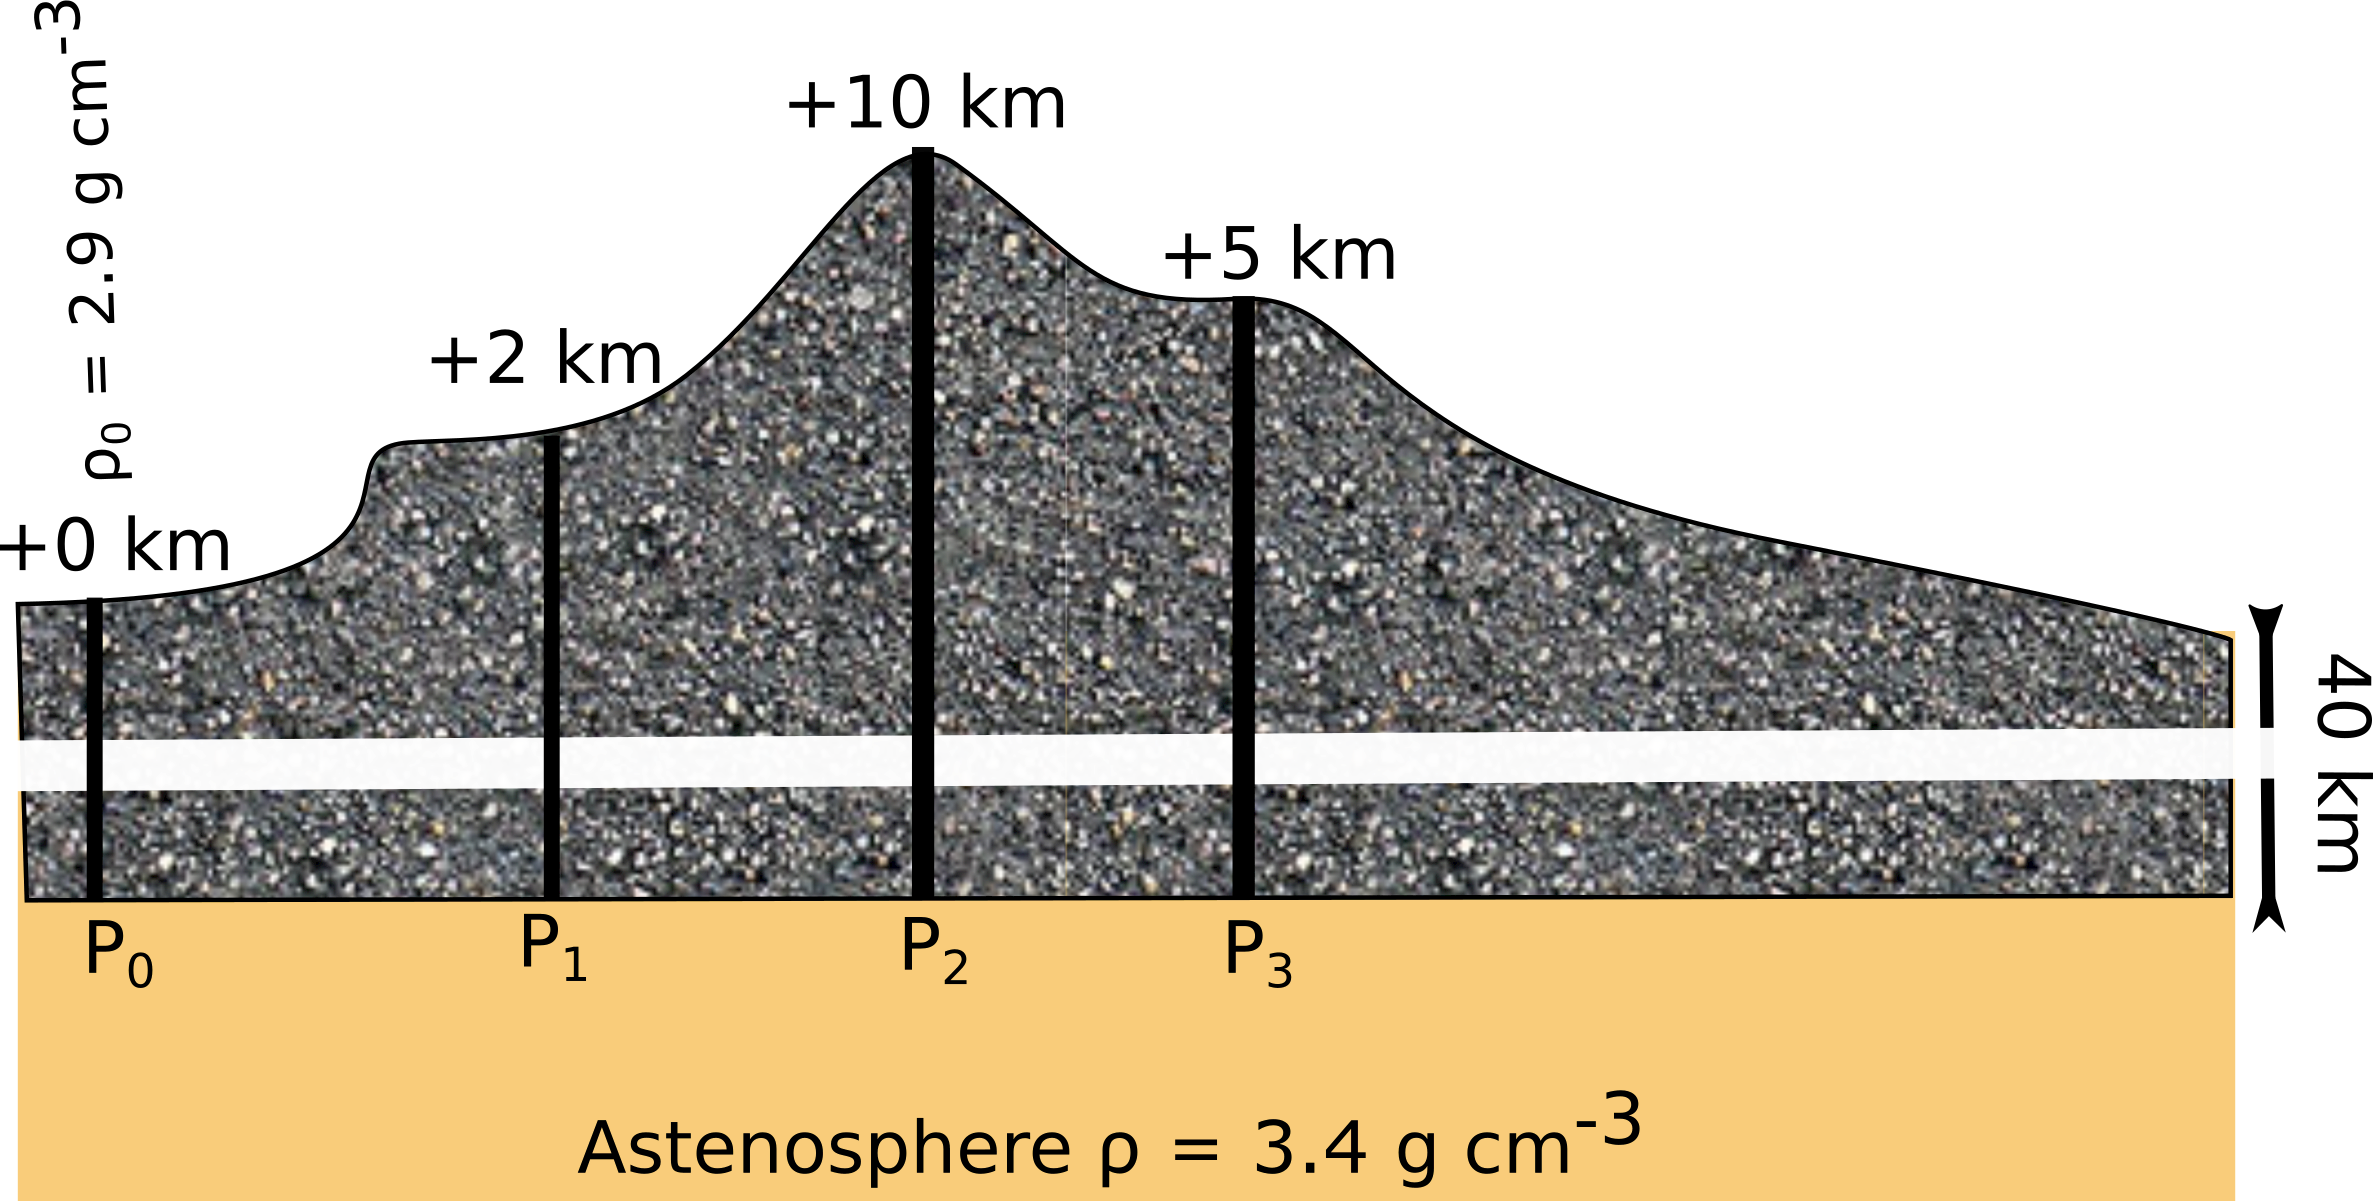
\includegraphics[width=0.5\textwidth]{Figures/Gravimetry/Pratt.png}
\end{center}

The figure above illustrates a crust with  with a inhomogenous density and a mountain change floating on the asthenosphere. Consider this as an idealised case in which every vertical slice is locally balanced (i.e. everything is in hydrostatic equilibrium which reduces to an effective 1D problem). Calculate the required densities in the vertical slices at $P_1 -- P_3$. (Tip: Below the crust the pressure is equal everywhere $P_1 -- P_3$)


\ifanswers
  \begin{tcolorbox}[enhanced jigsaw,breakable,pad at break*=1mm,
    colback=blue!5!white,colframe=babyblueeyes,title=Solutions]
The hydrostatic pressure $p$ at $P_1$ is $p ~ \rho g H_1$ with $H_1=40$~km. This is the same for the other locations. Hence:
\begin{align*}
\rho_0 H_1 &= \rho_1 (H_1 + 2) \\
\rightarrow \rho_1 &= \rho_0 \frac{H_1}{H_1+2} \approx 2.76 \, \text{g cm}^{-3}
\end{align*}
Equivalent for the other locations.
\end{tcolorbox}

\textbf{(b)}

\begin{center}
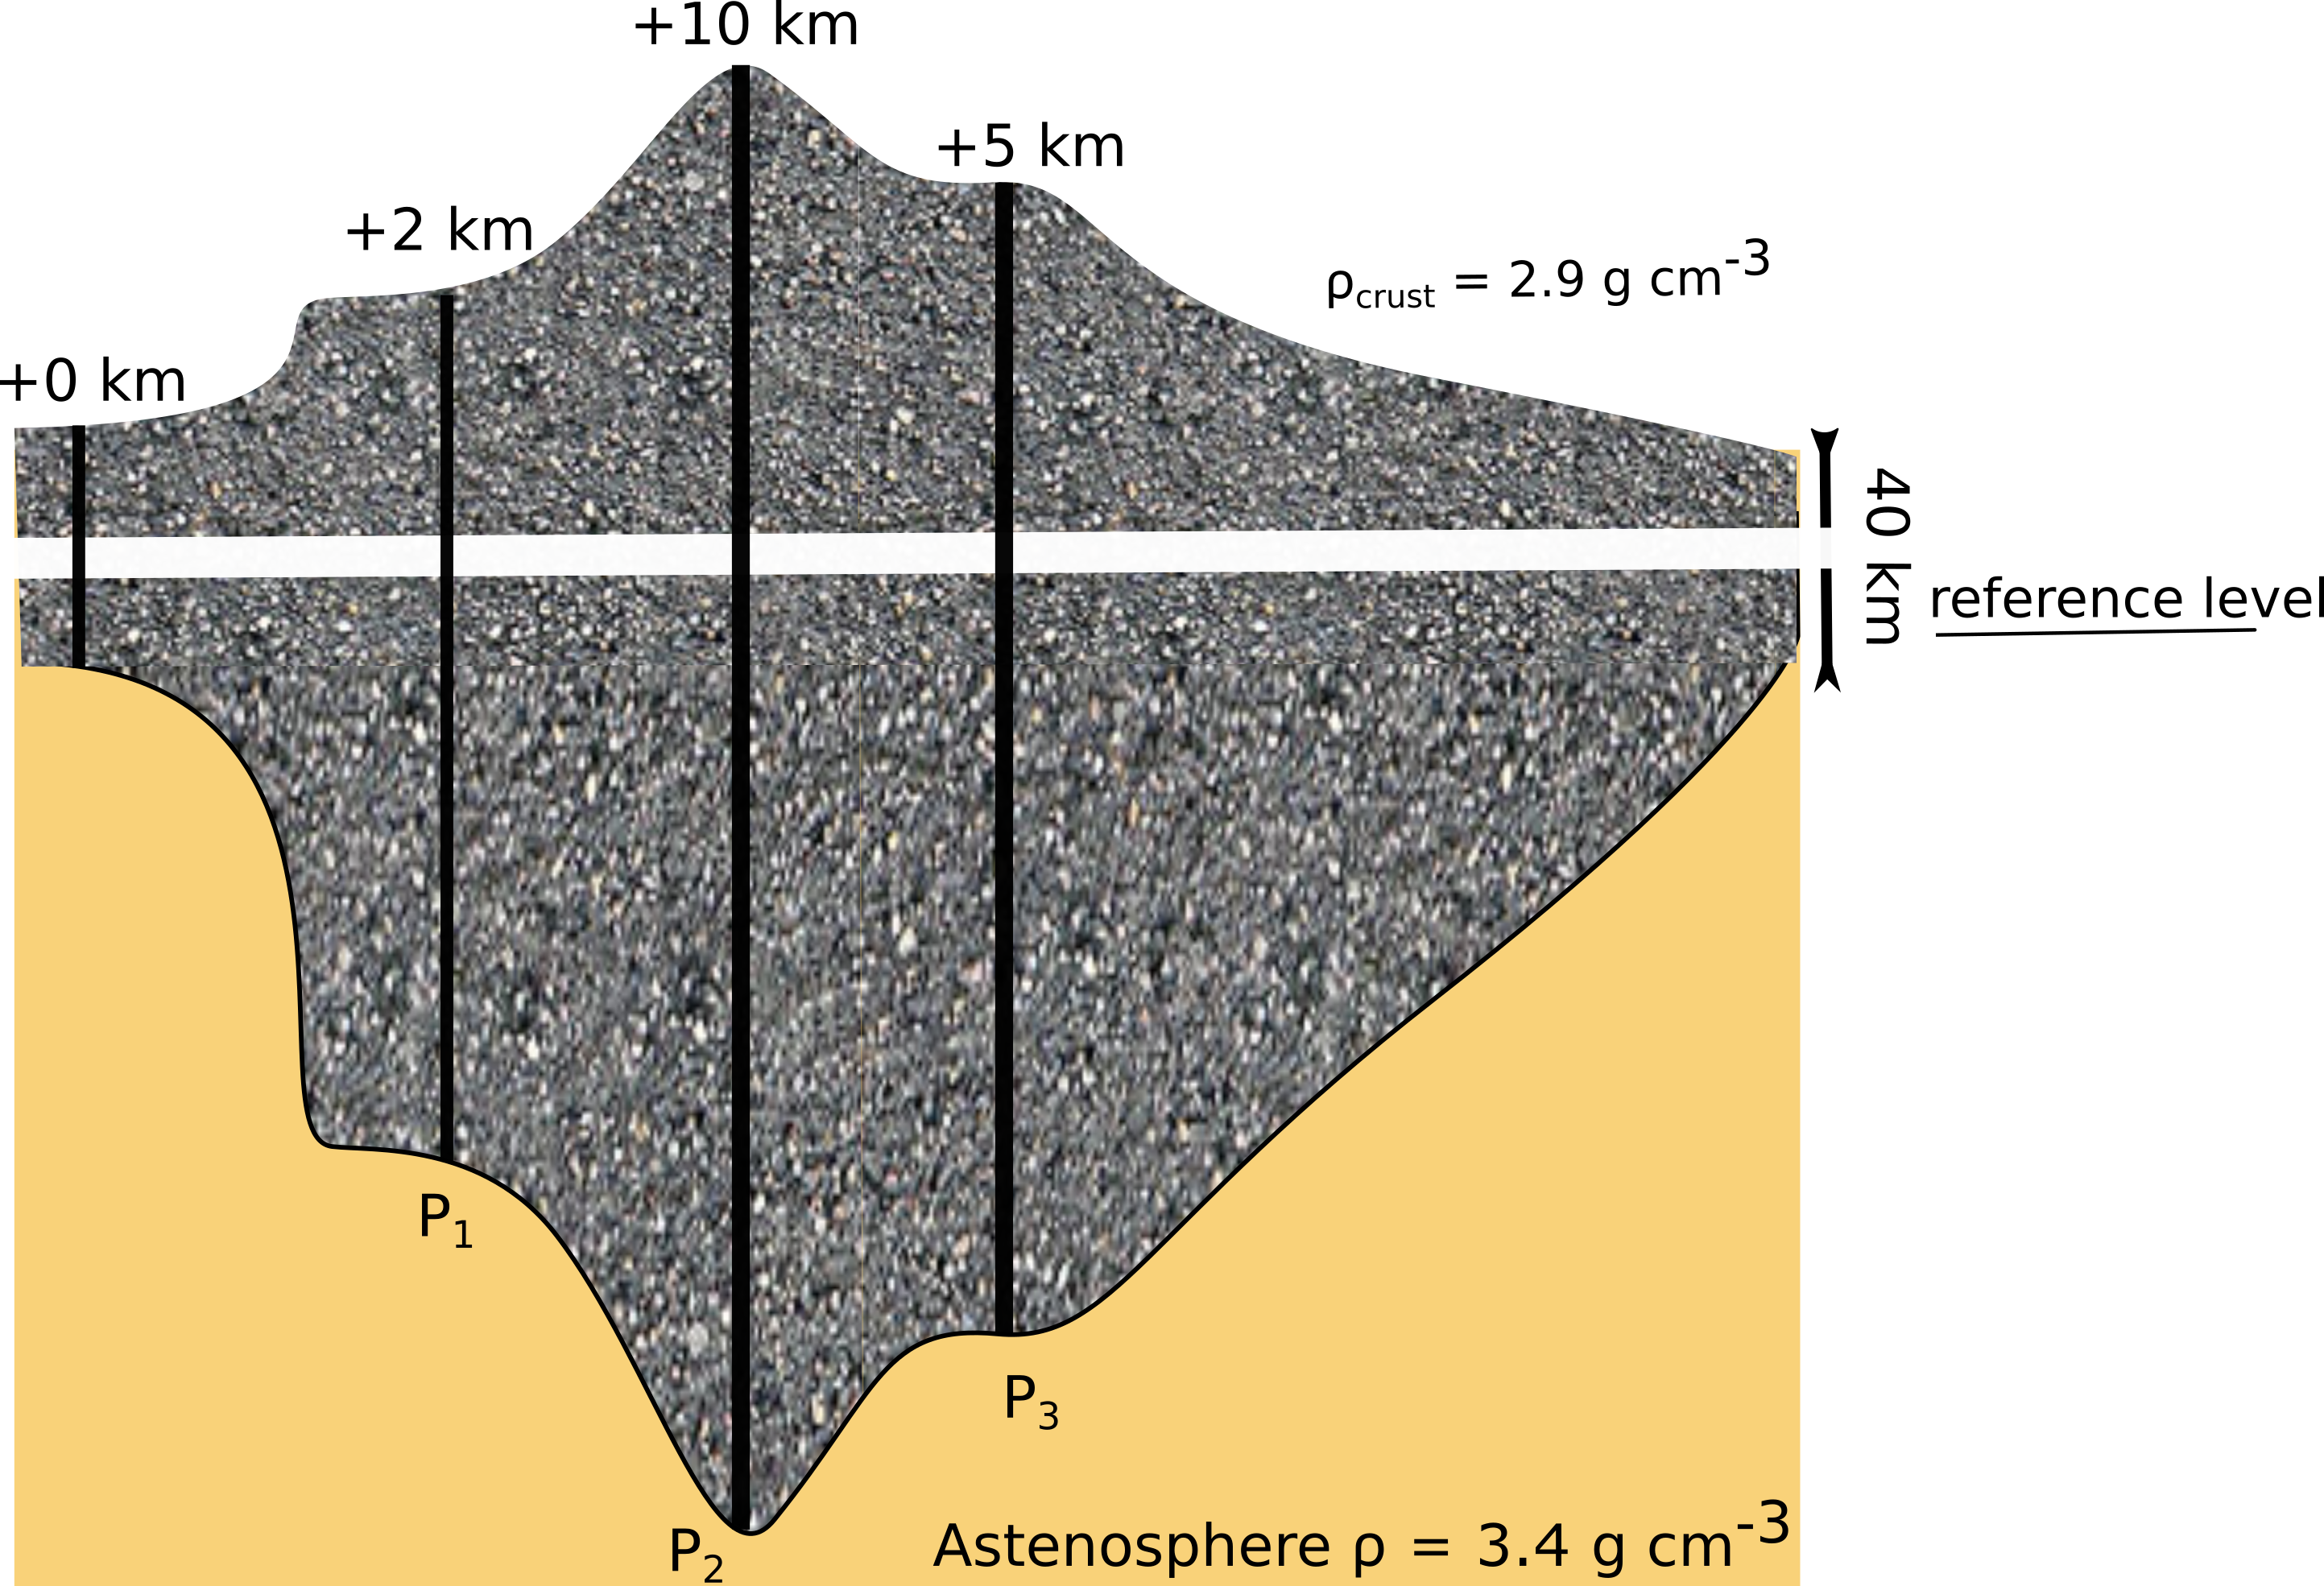
\includegraphics[width=0.5\textwidth]{Figures/Gravimetry/Airy.png}
\end{center}
\fi

The figure above illustrates a crust with a homogenous density and a mountain change floating on the asthenosphere. Consider this as an idealised case in which every vertical slice is locally balanced (i.e. everything is in hydrostatic equilibrium which reduces to an effective 1D problem). Calculate the thickness differences between $P_1 -- P_3$.


\ifanswers
  \begin{tcolorbox}[enhanced jigsaw,breakable,pad at break*=1mm,
    colback=blue!5!white,colframe=babyblueeyes,title=Solutions]
At the depth of $P_1$ we have:
\begin{align*}
\rho_c H_1 + \rho_A H_A &= \rho_c (H_1 + 2) \\
\rightarrow H_A &= 2 \frac{\rho_c}{\rho_A -\rho_c} \approx 11.6 \, \text{km}
\end{align*}
This means thickness at $P_1$ is 40 + 2 + 11.6 = 53.6 km. Equivalent for the other locations.
\end{tcolorbox}
\fi

\textbf{(c)} Draw an approximate profile for the free-air and the Bouger anomalies. How would this profile change if the mountain change is not in hydrostatic equilibrium? Which conclusions regarding the temporal evolution of the mountain chain would you draw from that? In which areas along this profile do you think is the assumption of local hydrostatic equilibrium most unlikely and how would this be reflected in the free-air anomaly?
\ifanswers
  \begin{tcolorbox}[enhanced jigsaw,breakable,pad at break*=1mm,
    colback=blue!5!white,colframe=babyblueeyes,title=Solutions]
    \begin{center}
    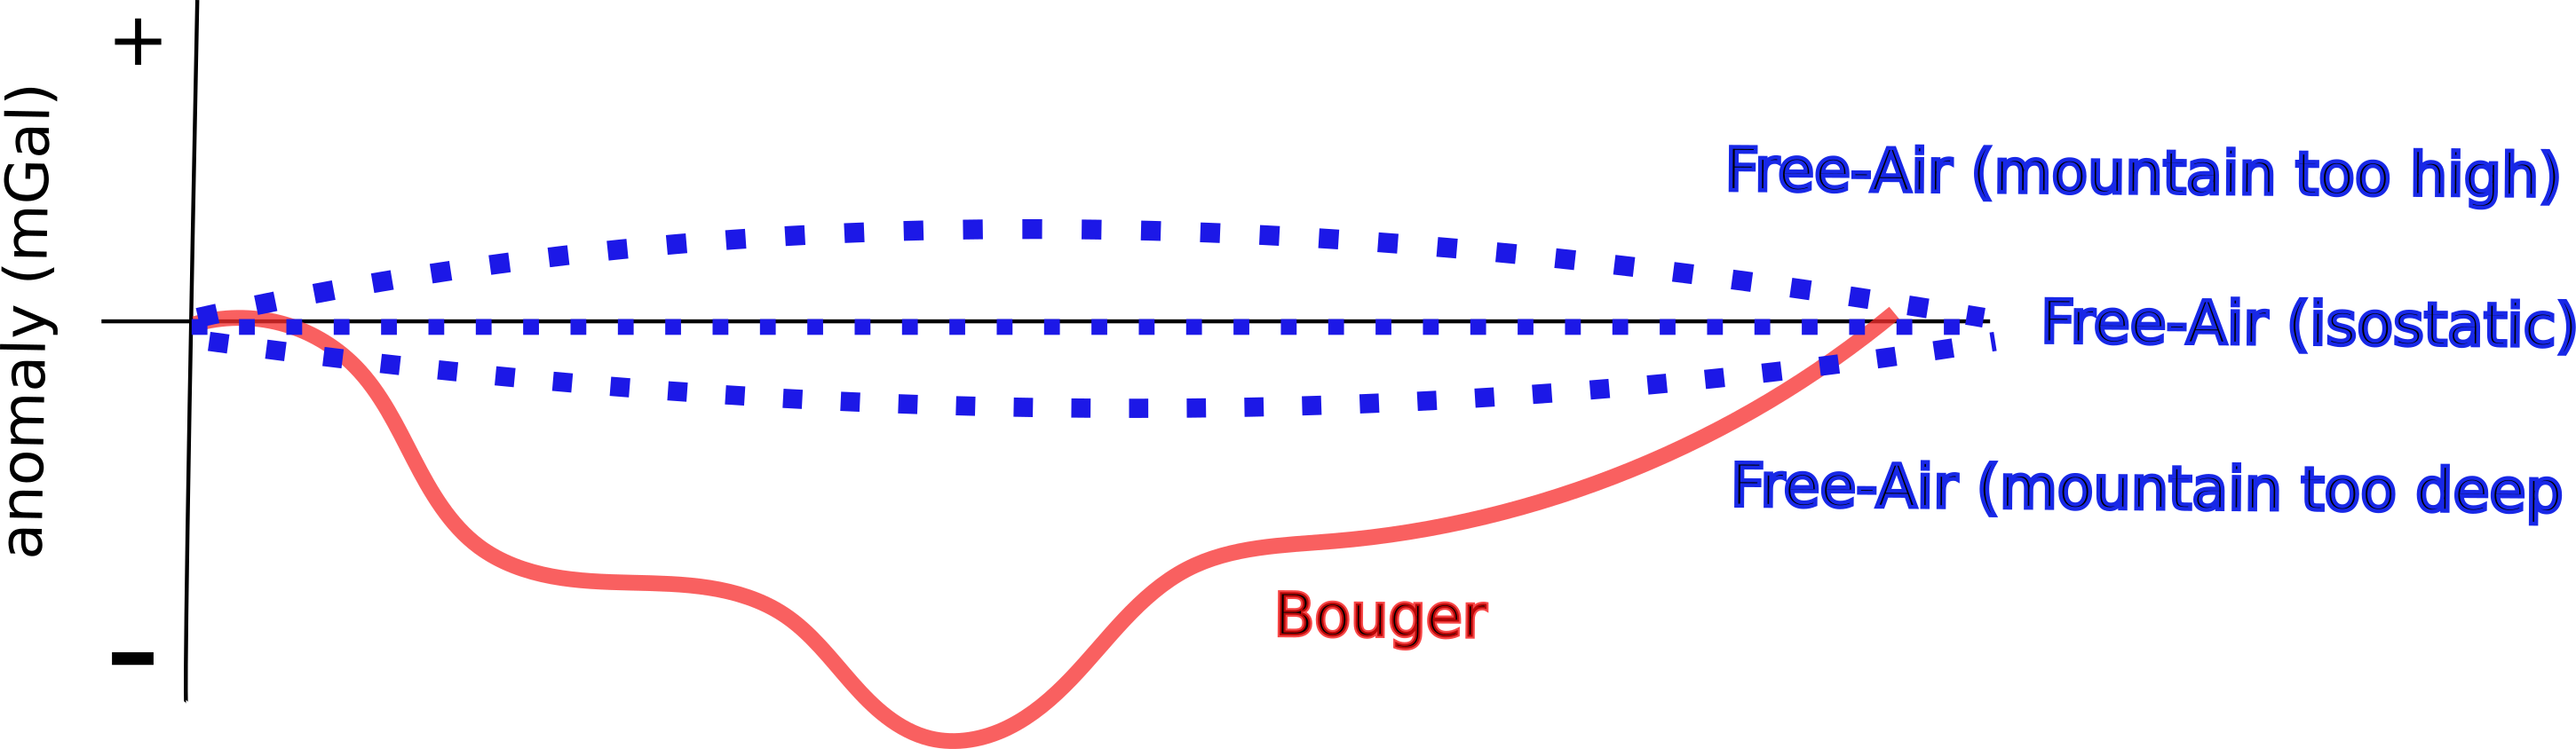
\includegraphics[width=0.9\textwidth]{Figures/Gravimetry/SolutionsProfiles.png}
    \end{center}
    \textbf{Text directly copied from: \href{https://www.geology.cwu.edu/facstaff/tim/TEACHING/Geophysics/gravity_geoid.pdf}{Link2PDF}}
    We can use gravity measurements to determine whether an area is in isostatic equilibrium. If a region is in isostatic equilibrium, there should be no gravity anomaly and hence no excess or lack of mass above the compensation depth. However, in practice, interpreting gravity measurements is a convoluted process. As an example, take the mountains shown above which are in 100\% isostatic compensation of the Airy type. The Bouguer anomaly across these mountains is negative, since below sea level there is a mass deficit under the mountains, ie, the low density root is holding the overlying mountains up. The Bouguer
    anomaly reflects the fact that the overlying mountains have been removed from the correction, which leaves only the mass deficit at depth unaccounted for, which causes the negative Bouguer anomaly. The free air anomaly, on the other hand, will be slightly positive, since this anomaly only takes into account the fact that we’re above sea level in our measurements and doesn’t take into account the distribution of mass below us. The slight positive reading comes from the fact that the overlying mountain is closer to us
    and and our point of measurement than is the compensating low density material at depth, and since gravitational acceleration drops off as $1/r^2$, the closer, mountain attraction io stronger than the more distant lack of attraction due to the mass deficit in the root, which results in a slight positive free air anomaly. The simplest way to determine whether a large-scale structure such as a mountain chain is in isostatic equilibrium is to use the free air anomaly. If a structure is totally compensated, away from the edges of the structure the free air anomaly will be very small. Near the edges is difficult to discern. If the structure is only partially compensated, the or not at all, then the free air anomaly will be strongly positive, up to several hundred millgals, while the Bouguer anomaly will be about zero. Free air anomalies are always almost isostatic anomalies. They do not tell you what type of compensation is ocurring (ie, Pratt versus Airy), but if compensation of any mechanism is complete, then the free air anomaly will be nearly zero.
  \end{tcolorbox}
\fi
%   \subsection{Forward modelling and non-uniqueness in potential field methods}
\begin{tcolorbox}[enhanced jigsaw,breakable,pad at break*=1mm,
  colback=blue!5!white,colframe=burgundy,title=Matlab (or Python),
  watermark color=white]
  Basic programming (Matlab/Python/R) will  likely be part of your study experience when you move to MSc level courses. It is a useful skill to have, but here we do not cover any introduction. What we do is that we start with codes that need  little user interaction to give you a feel for what programming can be about. In order to run this exercise you should have a working Matlab version on your Computer, please follow the installation instructions provided by the ZDV. Alternatively, we can also give you a laptop for the joint meeting.
\end{tcolorbox}
\label{Sec:GravityForwardModelling}
In order to predict how any kind of object will appear in a gravity survey, we need to solve the volume integral:
$$
 \vec{g}(r) = G\int \frac{1}{r^3} \rho(r) \vec{r} dV 
$$
which simplifies slightly to:
$$
 g_z(r) = G\int \frac{1}{r^2} \cos(\phi)\rho(r) dV = G\int \frac{z}{r^3} \rho(r) dV
$$
because often only the vertical component is of interest (same as in Ex 1.1).
However, the problem remains complicated as the integration bounds depend on the object's geometry and the integral needs to be solved for every $r$ along the gravimetry profile. Some solutions for special shapes you already know (e.g.sphere, bouger plate). Here we use the solution for a rectangular prism which fortunately others have already calculated for us (\textit{Naggy 1966, Geophysics VOL. XXX, SO. 2}). Using this solution, we can build up more complicated shapes out of individual prisms.

In the specific model applied individual prisms are defined with their widths in the horizontal (wx, wy) and the vertical (wz), together with the positions in the subsurface. The key is that the position coordinates (dx1, dx2, dy1, dy2, dz1, dz2) need to be prescribed relative to the measurement position which changes along the profile. The expected anomaly is then calculated based on the analytical solution.
\begin{enumerate}[label=(\alph*)]

  \item This exercises uses Matlab. However, only minimal Matlab skills are required to follow along. Download the files \textit{Gravimetry02\_ForwardModelling.m} and \textit{gravprism.m} into the same folder on your computer. Check out case 1 which simulates a rectangular object in the subsurface. Change it's location and size so that you know what is going on.

  \item Switch to case 2. This one treats the combined effect of two prisms. See what's different compared to case 1. Play around with positions to see what is going on.

  \item Switch to case 3. This one treats the individual effects of two prisms meaning that it doesn't sum them up. This one will not run until you fill out the parts marked with XXX. Use this case to illustrate that multiple situations in the sub-surface (e.g. a shallow prism with low density contrast vs. a lower prism with larger density contrast) can result in similar anomalies. This is an important finding. Forward models are often not unique, and therefore your interpretation won't be either. This situation occurs in many geophysical situations. Remember that.
\end{enumerate}
\ifanswers
\begin{tcolorbox}[enhanced jigsaw,breakable,pad at break*=1mm,
  colback=blue!5!white,colframe=babyblueeyes,title=Solutions,
  watermark color=white]
  \lstinputlisting[language=matlab]{../../Src/Gravimetry/PrismForwardModel/GravForwardModelPrismRD.m}
\end{tcolorbox}
\fi
%   \subsection{Some general questions to reflect on}
\textbf{1. Why does the mean sea level follow the shape of the Geoid?}
\ifanswers
  \begin{tcolorbox}[enhanced jigsaw,breakable,pad at break*=1mm,
    colback=blue!5!white,colframe=babyblueeyes,title=Solutions]
  Fluids cannot sustain shear stresses. If shear stresses exist the fluid surface will adjust so that the net force is normal to the surface. Without flow the gravitational field will therefore be perpendicular to the ocean surface, which is the definition of an equipotential line. The gravitational force along that line may vary.
  \end{tcolorbox}
\fi
\textbf{2. How can you describe the gravitational attraction between two point masses if none of them is located in the origin of the coordinate system applied?}
\ifanswers
  \begin{tcolorbox}[enhanced jigsaw,breakable,pad at break*=1mm,
    colback=blue!5!white,colframe=babyblueeyes,title=Solutions]
    $$
      \vec{F}(\vec{r}) = -GmM \frac{1}{||\vec{r}-\vec{r_0}||^2}\frac{\vec{r}-\vec{r}_0}{||\vec{r}-\vec{r}_0||}=-GmM \frac{1}{||\vec{r}-\vec{r_0}||^3}\vec{r}-\vec{r}_0
    $$
    \begin{center}
    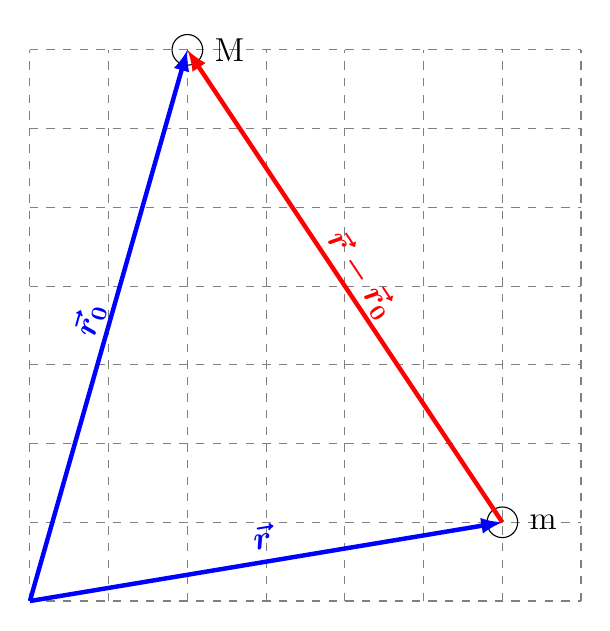
\begin{tikzpicture}[font=\boldmath]\large
      % Punkte
      \coordinate (O) at (0,0) {};
      \coordinate (A) at (6,1) {};
      \coordinate (B) at (2,7) {};
      % Draw the triangle
      % \filldraw (O) circle (3pt);
      % \filldraw (A) circle (7pt) node[sloped,midway, above] {$M$};
      % \filldraw (B) circle (3pt) node[sloped,midway, above] {$m$};
      \draw[dashed, gray] (0,0) grid (7,7);
      \node[draw,circle,label=right:m] (CircleNode) at (A)  {};
      \node[draw,circle=15pt,label=right:M] (CircleNode) at (B)  {};
      \draw[->, ultra thick, blue,   arrows={-latex}]  (O) -- (A) node[sloped,midway, above] {$\vec{r}$};
      \draw[->, ultra thick, blue,  arrows={-latex}]  (O) -- (B) node[sloped,midway,above=-0.1cm] {$\vec{r}_0$};
      \draw[->, ultra thick, red, arrows={-latex}]  (A) -- (B) node[sloped,midway,above=-0.1cm] {$\vec{r}-\vec{r}_0$};
  \end{tikzpicture}  
\end{center}
\end{tcolorbox}
\fi
\textbf{3. How does and equipotential line change by crossing an area of (a) mass deficit, and (b) mass excess?}
\ifanswers
  \begin{tcolorbox}[enhanced jigsaw,breakable,pad at break*=1mm,
    colback=blue!5!white,colframe=babyblueeyes,title=Solutions]
  For a mass deficit the gravitational vectors will point away from the anomaly. Therefore the corresponding equipotential lines is curved downwards. The opposite holds for a mass excess. I didn't figure out how to draw that yet in tikz.
  \end{tcolorbox}
\fi
  \textbf{4. Why do we have Earth \& Ocean tides? To understand the principle focus on the Moon's effect only.}
  \ifanswers
    \begin{tcolorbox}[enhanced jigsaw,breakable,pad at break*=1mm,
      colback=blue!5!white,colframe=babyblueeyes,title=Solutions]
    It comes down to two important effects: (1) The gravitational attraction of the moon towards the Earth is strong on the near-side than on the far side due to the $r^{-2}$ dependence. This alone leads to an ellipsoidal deformation. (2) The centrifugal acceleration due to the rotation around the center of mass between Earth and Moon counterbalances this to a certain extent. The formation of tidal bulges on either side of the Earth relative to the moon can be derived by decomposing the centrifugal acceleration into a radial component and a component that is perpendicular to the rotation axis. This leads to the lunar differential gravitational field that explains tidal bulges at both sides leading to semi-diurnal tides. The sun complicates this further but does not introduce different geophysical concepts. A detailed explanation can be found in Matsuda et al. 2015 (provided on Ilias).
    \end{tcolorbox}
  \fi
    \textbf{5. Discuss whether the sun or the moon is more important for tides.}
  
    \ifanswers
      \begin{tcolorbox}[enhanced jigsaw,breakable,pad at break*=1mm,
        colback=blue!5!white,colframe=babyblueeyes,title=Solutions]
        The sun is much larger and has a larger potential for tidal forces, however, it is also further away. The moon on the other hand has less weight but is closer. Doing the math shows that the sun accounts for about 40\% of the tidal forces on Earth.
      \end{tcolorbox}
\fi
      \textbf{6. Discuss the Airy and Pratt hypothesis. }



  % \setcounter{section}{2}
  % \section{Exercises for Magnetics 1}
  % \textbf{Version:} \today 
  
  % \textbf{Context:} Magnetics 01
  
  % \textbf{Timing:} All magnetics exercises should be completed by Thursday in week 5.
  %   \subsection{The magnetic dipole field}
\label{Sec:DipoleField}
Derive the two-dimensional dipole field $\vec{B}$ and its magnitude $|\vec{B}|$ from the potential field using:
\begin{align*}
    \vec{B} & = -\nabla A \\
       &\approx -\nabla \frac{|\vec{m}|\cos(\theta)}{r^2}
\end{align*}
and show that 
$$
    |B| = \frac{|\vec{m}|}{r^3}\sqrt{\left(3\cos^2(\theta) + 1\right)}
$$. 
Also show that: 
$$
    \nabla \cdot \vec{B} = 0.
$$
Discuss what this means in terms of the magnetic dipole field. Be aware that the gradient $\nabla$ and that the divergence $\nabla \cdot$ have a specific form in polar coordinates which you should look up. No need to memorize the specific form of these operators in different coordinate systems, but remember that they differ from coordinate system to coordinate system.


\ifanswers
    \begin{tcolorbox}[enhanced jigsaw,breakable,pad at break*=1mm,
    colback=blue!5!white,colframe=babyblueeyes,title=Solutions]
    We use the $\nabla$ operator in spherical coordinates:
    $$
        \nabla = \hat{r}\frac{\partial}{\partial r} + \hat{\theta} \frac{1}{r}\frac{\partial}{\partial \theta}
    $$
    The derivation with respect to $r$ is:
    $$ 
        \hat{r}\frac{\partial}{\partial r} \left(\frac{|\vec{m}|\cos(\theta)}{r^2}\right) = -2\frac{|\vec{m}|\cos(\theta)}{r^3}\hat{r}
    $$
    The derivation with respect to $\theta$ is:
    $$
    \hat{\theta} \frac{1}{r}\frac{\partial}{\partial \theta}\left(\frac{|\vec{m}|\cos(\theta)}{r^2}\right) = \frac{|\vec{m}|\sin(\theta)}{r^3}\hat{\theta}
    $$
    Taken together:
    $$
        \vec{B} = \frac{|\vec{m}|}{r^3}\left(2\cos(\theta)\hat{r} + \sin(\theta)\hat{\theta} \right)
    $$
    The norm of $|\vec{B}| = \sqrt{B_r^2 + B_{\theta}}$ as the unit vectors $\hat{r}$ and $\hat{\theta}$ are orthonormal. It is similar to a cartesian coordinate system but rotated.
    \begin{align*}
        &B_r^2 = \left(\frac{|\vec{m}|}{r^3}2\cos(\theta)\right)^2 \\ 
        &B_{\theta}^2 = \left(\frac{|\vec{m}|}{r^3} \sin(\theta) \right)^2 \\
        &B_r^2+ B_{\theta}^2 = \frac{|\vec{m}|^2}{r^6}\left(4\cos^2(\theta) + \sin^2(\theta)\right) \\
        &B_r^2+ B_{\theta}^2 = \frac{|\vec{m}|^2}{r^6}\left(3\cos^2(\theta) + 1\right) \\ 
        &\sqrt{B_r^2+ B_{\theta}^2} = \frac{|\vec{m}|}{r^3}\sqrt{\left(3\cos^2(\theta) + 1\right)} \\
    \end{align*}
    For the divergence we use $\nabla \cdot \vec{B} = \frac{1}{r^2}\frac{\partial}{\partial r}\left( \right)$
    \end{tcolorbox}
\fi

  %   \subsection{The Earth's magnetic field}
Use online resources and characterize the Earth's magnetic field in Tübingen in terms of (declination, inclination, horizontal component, total field strength etc.). Can you find information about temporal variability? How large is it and over which time frame? Visualize the time series. Post values and graphics in the forum.

\ifanswers
    \begin{tcolorbox}[enhanced jigsaw,breakable,pad at break*=1mm,
    colback=blue!5!white,colframe=babyblueeyes,title=Solutions]
        %\begin{figure}[h!]
            \begin{center}
            \begin{tikzpicture}
                \begin{axis}[
                    width=\linewidth, % Scale the plot to \linewidth
                    grid=major, % Display a grid
                    grid style={dashed,gray!30}, % Set the style
                    ylabel=Total Intensity (nT), % Set the labels
                    xlabel=Decimal Year,
            %      x unit=none, % Set the respective units
            %     y unit=none,
            %     legend style={at={(0.5,-0.2)},anchor=north}, % Put the legend below the plot
            %     x tick label style={rotate=0,anchor=east} % Display labels sideways
                ]
                \addplot 
                % add a plot from table; you select the columns by using the actual name in
                % the .csv file (on top)
                table[x=DecimalYear,y=Total,col sep=comma] {/Users/rdrews/Nextcloud/esd_teach/geophyscis_BSc_SoSe22/Exercises/All/Includes/Magnetics/data/igrfwmmData_nh.csv}; 
                \legend{IGRF}
                \end{axis}
            \end{tikzpicture}
        %    \caption{Total field variation as function of decimal year from 1969 to 2022 using the IGRF model.}
            \end{center}
        %\end{figure}
        Declination Inclination Horizontal Intensity NorthComp East Comp Vertical Comp TotalField
        3.2940 	64.4662 	20,937.4 nT 	20,902.8 nT 1,203.1 nT 	43,829.7 nT 	48,573.8 nT
    \end{tcolorbox}
    \fi

  % \subsection{Preparation for report writing}
  % Read the document Geophysics\_Report\_Suggestions provided under general documents on Ilias. Provide feedback from other report-writing experiences if you have any.

  % \setcounter{section}{3}
  % \section{Exercises for Magnetics 2}
  % \textbf{Version:} \today 
  
  % \textbf{Context:} Magnetics 01 + 02
  
  % \textbf{Timing:} All magnetics exercises should be completed by Thursday in week 5.
  % \subsection{Natural Magnetic Remanence}
\label{Sec:Remanence}
Some rocks and other materials show a remanent magnetization additional to the induced magnetization by the contemporary Earth's magnetic field. The total magnetic moment is the superposition of the two. This has important implications for the interpretation of magnetic anomalies (see below), but can also be exploited for a number of important findings in paleomagnetics shaping our understanding of processes in the Earth System. Find an applications in which remanence helps us to understand the Earth's history (e.g., in terms of plate tectonics or dating) and post a short snapshot (pictures, key messages) of this in the forum. Don't post it if somebody else already did.


  %   \subsection{Forward Modelling of a Dipole}
\label{Sec:MagForwardModel}
 and that the divergence $\nabla \cdot$ have a specific form in polar coordinates which you should look up. No need to memorize the specific form of these operators in different coordinate systems, but remember that they differ from coordinate system to coordinate system.


\ifanswers
    \begin{tcolorbox}[enhanced jigsaw,breakable,pad at break*=1mm,
    colback=blue!5!white,colframe=babyblueeyes,title=Solutions]
    
    Tübingen (Morgenstelle) is located at 48.537624 N 9.031300 E (342 m.a.s.l.). Using NOAA's magnetic field caluclator (\url{https://www.ngdc.noaa.gov/geomag/calculators/magcalc.shtml#igrfwmm})
\fi

  %   \subsection{General Questions}
\label{Sec:MagGeneralQuestions}

\begin{enumerate}[label=(\alph*)]
    \item In magnetic surveys often the vertical gradient is determined by measuring with two sensors installed at different heights let's say 0.5 meters apart. Develop an argument (including drawings or results from forward modeling) why this type of survey emphasizes near-surface targets.
    \item Compare the gravity method with the magnetic method using the table below. 
\end{enumerate}

\begin{tabularx}{\textwidth}{X|X X}
    \centering
%  \begin{tabular}{l{3cm}|c c}
     & Gravity Method & Magnetic Method \\
 \hline
 active or passive &  &   \\ \specialrule{0.5pt}{10pt}{1pt}
 geophysical parameter &   &   \\ \specialrule{0.5pt}{1pt}{1pt}
 potential field  & & \\ \specialrule{0.5pt}{1pt}{1pt}
 time variability of earth's field &  &  \\ \specialrule{0.5pt}{1pt}{1pt}
 typical data processing &  &   \\ \specialrule{0.5pt}{1pt}{1pt}
 basic source types &  &  \\ \specialrule{0.5pt}{1pt}{1pt}
 field characteristics &  &  \\ \specialrule{0.5pt}{1pt}{1pt}
 force characterisitcs &  &  \\ \specialrule{0.5pt}{1pt}{1pt}
 sensors &  &  \\ \specialrule{0.5pt}{1pt}{1pt}
 use of reference station &  &  \\ \specialrule{0.5pt}{1pt}{1pt}
 applications & &    %  \end{tabular}
%  \caption{Blabla}
%  \label{tab:1}
\end{tabularx}

\ifanswers
\begin{tcolorbox}[enhanced jigsaw,breakable,pad at break*=1mm,
    colback=blue!5!white,colframe=babyblueeyes,title=Solutions]
\textbf{(a)} In general, the deeper the magnetic source, the broader and gentler the gradients of the resulting anomaly will be (see forward modeling). Also, in general, the shallower the magnetic object, the sharper and narrower the resulting anomaly. The gradient picks this rapid changes up an amplifies them.

\textbf{(b)}


    \begin{tabularx}{\textwidth}{X|X X}
        \centering
    %  \begin{tabular}{l{3cm}|c c}
            & Gravity Method & Magnetic Method \\
        \hline
        active or passive & passive & passive  \\ \specialrule{0.5pt}{1pt}{1pt}
        geophysical parameter & density ($\rho$) & magnetic susceptibility ($\chi$)  \\ \specialrule{0.5pt}{1pt}{1pt}
        potential field  & $\vec{g}=-\nabla \phi$ & $\vec{B}=-\nabla A$ \\ \specialrule{0.5pt}{1pt}{1pt}
        time variability of earth's field & slow \& small (e.g. tides) & strong \& fast (e.g., space weather) \\ \specialrule{0.5pt}{1pt}{1pt}
        typical data processing & latitudinal, elevation, terrain, bouger corrections &  interpretation in terms of ambient field, gradiometry \\ \specialrule{0.5pt}{1pt}{1pt}
        basic source types & point mass & magnetic dipole from current loop \\ \specialrule{0.5pt}{1pt}{1pt}
        field characteristics & spherically symmetric, $1/r^2$ decay & dipole field, closed field lines, $1/r^2$ decay for monopole, $1/r^3$ for dipoles \\ \specialrule{0.5pt}{1pt}{1pt}
        force characterisitcs & attractive & attractive or repulsive \\ \specialrule{0.5pt}{1pt}{1pt}
        sensors & springs, free-fall, pendulum & proton precession $T$, fluxgate $\vec{B}$, optically pumped \\ \specialrule{0.5pt}{1pt}{1pt}
        use of reference station & yes, mostly due to sensor drift & yes, due to secular variability \\ \specialrule{0.5pt}{1pt}{1pt}
        applications & ice-sheet mass balance, groundwater variability, sediment infill valley,..& mid-ocean ridges, pipes, paleochronology, tectonics   %  \end{tabular}
    %  \caption{Blabla}
    %  \label{tab:1}
    \end{tabularx}
\end{tcolorbox}
\fi

  %   \subsection{Interpolation of scattered data}
\label{Sec:Interpolation}
Download the datafile \textit{LonLatXYZ.txt} from Ilias. This is data collected witha GPS from a topographic survey in Antarctica. It is an ASCII txt file with longitude, latitude, polar sterographic, polar stereographic y, and elevation (relative to ellipsoid). Find a way how you can interpolate the data to visualize the landscape. You could use Matlab, Python or a GIS. We try to help where we can. 

\ifanswers
\begin{tcolorbox}[enhanced jigsaw,breakable,pad at break*=1mm,
    colback=blue!5!white,colframe=babyblueeyes,title=Solutions]
    \lstinputlisting[language=matlab]{../../Src/Exercises/Magnetics/GriddingRD.m}
\end{tcolorbox}
\fi

    \setcounter{section}{4}
    \section{Exercises for Resistivity Method 1}
    \textbf{Version:} \today 
    
    \textbf{Context:} Resistivity Method 01
    
    \textbf{Timing:} All resistivity exercises should be completed the latest by June 4th 2022
    \subsection{Resistivity Survey in a Sandbox}
\begin{figure}[th]
    \centering
    \includegraphics*[width=0.5\textwidth]{Figures/Resistivity/Sandbox.png}
    \caption{Toy setup for understanding the principles of the resistivity method.}
\end{figure}
\begin{tcolorbox}[enhanced jigsaw,breakable,pad at break*=1mm,
    colback=blue!5!white,colframe=burgundy,title=Group Work,
    watermark color=white]
    Self-organize with your groups to do this during our contact time on Thursdays. Ideally two to three groups should do the experiment in a total of 2h. We will assign two sessions for that. After you are done, disconnect all cables and keep everything as you found it for the next group. \textbf{When using the battery with open-end cables, be careful that you do not short them.}
\end{tcolorbox}
(\textit{practical}) Use a battery, four electrodes and two multimeters to determine the apparant resistivity of sand in a sandbox. You can align the electrodes in a co-linear Wenner array and also check how/if the resistivity changes with variable array types and moisture content. Post your results in the forum and compare them with  the literature values. Don't overestimate the accuracy here, it is more about internalizing the measurement principle and to strengthen your cabling skills.  All material (Fig. 1) will be provided on-site. 

\ifanswers
    \begin{tcolorbox}[enhanced jigsaw,breakable,pad at break*=1mm,
    colback=blue!5!white,colframe=babyblueeyes,title=Solutions,
    watermark color=white]
    Discussions on site and video online.
    \end{tcolorbox}
\fi

    \subsection{The LaPlace Equation}
(\textit{easy}) In the lecture we derived that the potential field of a single electrode (second electrode is located at infinity) satisfies the LaPlace equation:
$$
\vec \nabla^2 V = \Delta V = 0.
$$
Show that our \textit{Ansatz} $V(r) = \frac{A}{r}$ satisfies this equation in spherical coordinates. Note that the LaPlace in spherical coordinates is $\nabla^2 = \frac{1}{r^2}\frac{\partial }{\partial r}\left(r^2\frac{\partial }{\partial r}\right)$.

\ifanswers
    \begin{tcolorbox}[enhanced jigsaw,breakable,pad at break*=1mm,
    colback=blue!5!white,colframe=babyblueeyes,title=Solutions,
    watermark color=white]
    \begin{eqnarray*}
    \nabla^2 &=& \frac{1}{r^2}\frac{\partial }{\partial r}\left(r^2\frac{\partial }{\partial r}\frac{A}{r}\right)   \\
    &=& \frac{1}{r^2}\frac{\partial }{\partial r}\left(-r^2 \frac{A}{r^2}\right) \\
    &=& \frac{1}{r^2}\frac{\partial }{\partial r} A = 0
    \end{eqnarray*}
    \end{tcolorbox}
\fi
    \subsection{Depth of Investigation}
\begin{center}
\begin{tikzpicture}
      
    \newcommand\EMF{\mathcal{E}};
    \colorlet{Icol}{blue!50!black}
    \colorlet{Ccol}{orange!90!black}
    \colorlet{Rcol}{red}
    \colorlet{loopcol}{red!90!black!25}
    \colorlet{pluscol}{red!60!black}
    \colorlet{minuscol}{blue!60!black}
    \tikzstyle{EMF}=[battery1,l=$\EMF$];
    \tikzstyle{internal R}=[R,color=Rcol,Rcol,l=$r$,/tikz/circuitikz/bipoles/length=30pt];
    \tikzstyle{loop}=[->,red!90!black!25];
    \tikzstyle{loop label}=[loopcol,fill=white,scale=0.8,inner sep=1];
    \tikzstyle{thick R}=[R,color=Rcol,thick,Rcol,l=$R$];
    
    \begin{scope}[rotate=-90,transform shape]
      \fill[pattern = crosshatch dots,pattern color = brown!80!red] (0.0,-0.5) rectangle ++(6,11);
     % \node[rotate=90] at (0.25,1.5) {Surface};
      \draw (0,0)
      %to[R,color=Rcol,thick,l={{{{\rotatebox[origin=c]{90}{$R_{c2}$}}}}}] (6,9) 
      %to[R,color=Rcol,thick,l={{{{\rotatebox[origin=c]{90}{$R$}}}}}] (6,0) 
      %to[R,color=Rcol,thick,l={{{{\rotatebox[origin=c]{90}{$R_{c1}$}}}}}] (0,0) 
      to [ammeter, color=black] (0,9);
      \node[rotate=90,above] at (0,9) {$B$};
      \node[rotate=90,above] at (0,0) {$A$};
 
     % \node[rotate=90] at (0,4) {$\Delta V$};
        %  \draw[->,red] (0.5, 2.15) --++ (1.2,0) node[midway,above=1] {current $I$};
        %  \draw[->,red] (0.5,-0.15) --++ (1.2,0) node[midway,below=1] {electron flow};
      \end{scope}
    %   \draw[-,color=black] (2,-0.8) -- (2,1.2);
    %   \draw[-,color=black] (2,1.2) -- node[above] {$\Delta$ U} (5,1.2);
    %   \draw[-,color=black] (5,1.2) -- (5,-0.8);
      \draw[<->,color=blue,line width=0.75mm] (3,1.5) -- (0.0,1.5) node[midway,below] {$x$};
      \draw[<->,color=blue,line width=0.75mm] (3.0,1.5) -- (9.0,1.5) node[midway,below] {$x-L$};
      \draw[<->,color=blue,line width=0.75mm] (3.0,1.5) -- (9.0,1.5) node[midway,below] {$x-L$};
      \draw[<->,color=blue,line width=0.75mm] (0.0,0.9) -- (9.0,0.9) node[midway,below] {$L$};
      \draw[-,color=black,dashed,,line width=0.75mm] (3.0,0.0) -- (3.0,-6);
      \draw[-,color=black,line width=0.75mm] (0.0,0.0) -- (3.0,-4) node[midway,sloped,above] {$r_1$};
      \draw[-,color=black,line width=0.75mm] (0.0,0.0) -- (3.0,-4) node[midway,sloped,above] {$r_1$};
      \draw[-,color=black,line width=0.75mm] (9,0) -- (3.0,-4) node[midway,sloped,above] {$r_2$};
      \draw[->,color=black,line width=1.0mm] (2.5,-2.1) -- (3.5,-2.1) node[left,above] {$J_x$};
      \draw[->,color=black,line width=1.0mm] (2.5,-3.1) -- (3.5,-3.1) node[left,above] {$J_x$};
      \draw[->,color=black,line width=1.0mm] (2.5,-4.1) -- (3.5,-4.1) node[left,above] {$J_x$};
      \draw[->,color=black,line width=1.0mm] (2.5,-5.1) -- (3.5,-5.1) node[left,above] {$J_x$};
    %   \node[above] at (2,1.2) {$M$};
    %   \node[above] at (5,1.2) {$N$};
  \end{tikzpicture}
\end{center}
(\textit{tricky}) In this exercise we would like to approximate which depth interval the resistivity method is sensitive to. We already understand intuitively that a larger electrode spacing between A and B increases the depth penetration. Here we aim to do it quantitatively. For this we consider a vertical plane located at distance $x$ away from electrode A, and calculate how much of the current flow density crosses that plane. This means we would like to calculate $J_x(z)$. From the lecture we know that:

$$
\vec{j} = \sigma \vec{E} = \sigma \nabla V \rightarrow J_x = -\frac{I}{2\pi} \frac{\partial }{\partial x} \left(\frac{1}{r_1} - \frac{1}{r_2}\right )
$$
Adopting the coordinate system from the Figure above we choose $r_1 =\sqrt{x^2+y^2+z^2}$ with z point along depth and y into the plane. First calculate $J_x$ for any point P, then show that 
$$
J_x (x=L/2) = \frac{I}{2\pi}\frac{L}{(z^2+y^2+\frac{L^2}{4})^{3/2}}
$$
at the center point. Sketch this function roughly on paper for a fixed L. Now consider a fixed layer at constant depth $z$. How does $J_x$ change as $L$ is varied? Show that $J_x(x=L/2,z)$ has a maximum at $L=\sqrt{2}{z}$. This shows that depth penetration increases as we increase the distance between the current electrodes A and B. Still, most of the current flow will be near the surface. In order to define a depth of investigation we will need to apply some thresholding and include placement of the M,N electrodes. This varies from array to array.
\ifanswers
    \begin{tcolorbox}[enhanced jigsaw,breakable,pad at break*=1mm,
    colback=blue!5!white,colframe=babyblueeyes,title=Solutions,
    watermark color=white]
   
   
 
      Calculation of the derivative is:
      \begin{eqnarray*}
        &-\frac{I}{2\pi} \frac{\partial }{\partial x} \left(\frac{1}{r_1} - \frac{1}{r_2}\right) =  \\
        &-\frac{I}{2\pi} \frac{\partial }{\partial x} \left(\frac{1}{\sqrt{x^2+y^2+z^2}} - \frac{1}{\sqrt{(x-L)^2+y^2+z^2}}\right)= \\
        &\frac{I}{4\pi}  \left(\frac{2x}{(x^2+y^2+z^2)^{3/2}} - \frac{2(x-L)}{((x-L)^2+y^2+z^2)^{3/2}}\right)= \\
        &\frac{I}{2\pi}  \left(\frac{x}{(x^2+y^2+z^2)^{3/2}} - \frac{(x-L)}{((x-L)^2+y^2+z^2)^{3/2}}\right)
     \end{eqnarray*}
     Now consider this for the center at $x=\frac{L}{2}$ where $r_1 = r_2 = \sqrt{L^2/4+y^2+z^2}$:
     \begin{eqnarray*}
      &J_x(x=L/2) =   \\
      & \frac{I}{2\pi}\left(\frac{L/2}{(L^2/4+y^2+z^2)^{3/2}} + \frac{(L/2)}{(L^2/4+y^2+z^2)^{3/2}}\right) = \\
      &\frac{I}{2\pi}  \left(\frac{L}{(L^2/4+y^2+z^2)^{3/2}}\right)
     \end{eqnarray*}
     \begin{center}
     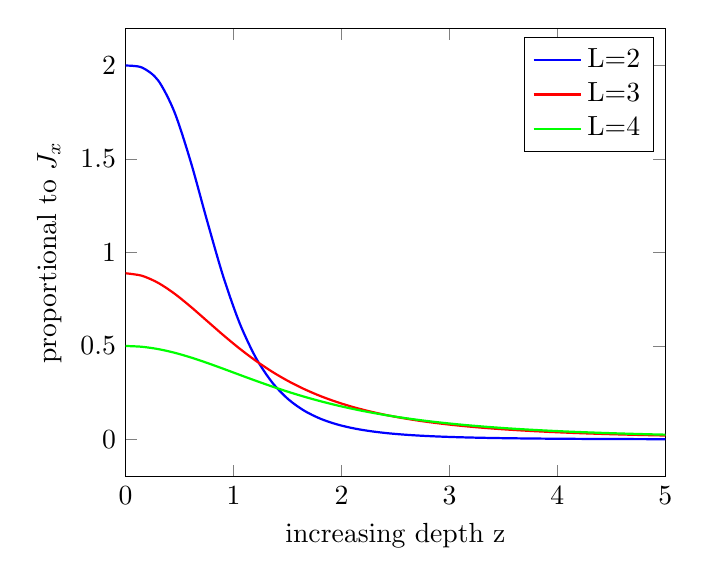
\begin{tikzpicture}
     \begin{axis}[
      xmin = 0, xmax = 5,xlabel=increasing depth z,
      ylabel={proportional to $J_x$}]
      \addplot[
          domain = 0:30,
          samples = 200,
          smooth,
          thick,
          blue,
      ] {2/(x^3+2*2/4)^(3/2)};
      \addplot[
        domain = 0:30,
        samples = 200,
        smooth,
        thick,
        red,
    ] {3/((x^2+3*3/4)^(3/2))};
    \addplot[
      domain = 0:30,
      samples = 200,
      smooth,
      thick,
      green,
     ] {4/((x^2+4*4/4)^(3/2))};
  \legend{L=2,L=3,L=4}
  \end{axis}
\end{tikzpicture}
\end{center}
Next we calculate the derivative with respect to $L$ (at x=L/2 and y=0):
\begin{eqnarray*}
  \frac{\partial}{\partial L}\left(\frac{L}{(L^2/4+z^2)^{3/2}}\right) = 0 \\
  (L^2/4+z^2)^{-3/2} -\frac{3}{2}L (L^2/4+z^2)^{-5/2}L/2 = 0 \\
  1 -\frac{3}{4}L^2 (L^2/4+z^2)^{-1} = 0 \\
  \rightarrow L^2/4+z^2 = \frac{3}{4}L^2 \\
  \rightarrow -L^2/2+z^2 = 0 \\
  \rightarrow L^2 = 2 z^2 \\
  \rightarrow L = \sqrt{2} z \\
\end{eqnarray*}

\begin{center}
  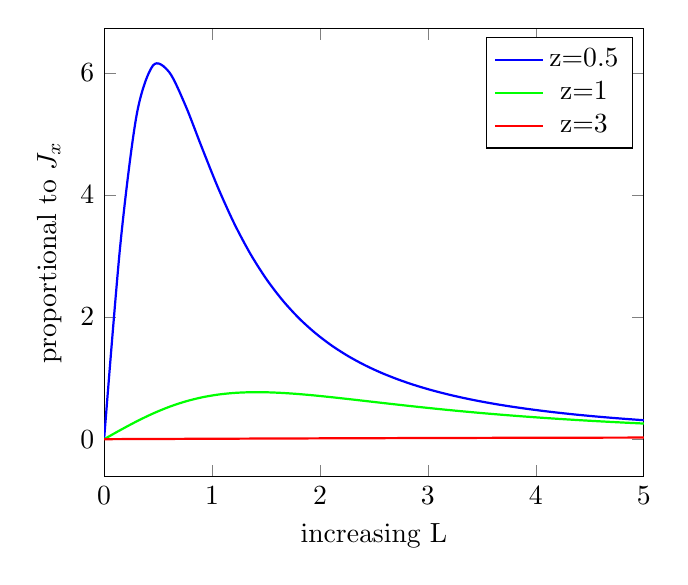
\begin{tikzpicture}
  \begin{axis}[
   xmin = 0, xmax = 5,xlabel=increasing L,
   ylabel={proportional to $J_x$}]
   \addplot[
       domain = 0:30,
       samples = 200,
       smooth,
       thick,
       blue,
   ] {x/(0.5^3+x*x/4)^(3/2)};
   \addplot[
    domain = 0:30,
    samples = 200,
    smooth,
    thick,
    green,
] {x/(1^3+x*x/4)^(3/2)};
\addplot[
  domain = 0:30,
  samples = 200,
  smooth,
  thick,
  red,
] {x/(3^3+x*x/4)^(3/2)};
 \legend{z=0.5,z=1,z=3}
\end{axis}
\end{tikzpicture}
Normalized in Telford chapter 8.
\end{center}

\end{tcolorbox}

\fi

    
    \setcounter{section}{5}
    \section{Exercises for Resistivity Method and Induced Polarization}
    \textbf{Version:} \today 
    
    \textbf{Context:} Resistivity Method 02, Induced Polarization 01 \& Self-Potential 01
    
    \textbf{Timing:} All resistivity exercises should be completed the latest by June 13th 2022
    \subsection{Forward Modelling of a vertical electrical sounding survey}
(a) Use the attached file \textit{RD\_VES\_ForwardModel\_Ex6.ipynb} which contains a Jupyter Notebook with PyGimli as discussed in the latest video. Set-up a sub-surface model with three different resistivities for cases:
\begin{itemize}
    \item $ \rho_1 > \rho_2 > \rho_3$
    \item $ \rho_1 < \rho_2 < \rho_3$
    \item $ \rho_1 < \rho_2, \rho_2 > \rho_3$
\end{itemize}
Also explore possibilities of four layers cases. This type of forward modelling can be useful for your applied exercises in geoelectrics.

(b) Change the Jupyter notebook code so that you can visualize output from two forward runs (use a copy and past where you can). Illustrate to different sub-surface models which result in a similar vertical electrical sounding observations. Memorize that does ambiguities (same as, e.g., for gravity surveys) are very prevalent in geophysical applications.
\ifanswers
    \begin{tcolorbox}[enhanced jigsaw,breakable,pad at break*=1mm,
    colback=blue!5!white,colframe=babyblueeyes,title=Solutions,
    watermark color=white]
    %\lstinputlisting[language=python]{../../Src/Resistivity/RD_VES_ForwardModel_Ex6Solution.ipynb}
    ../../Src/Resistivity/RD\_VES\_ForwardModel\_Ex6Solution.ipynb
    \end{tcolorbox}
\fi
    \subsection{Geoelectric Array Types}
(a) Show explicitly that for a Wenner ($\alpha$) array the geometry factor is $K = 2\pi a$ where $a$ is the distance between between all electrodes.

(b) In preparation of the applied exercises, make a table with the different array types (Wenner $\alpha$, Schlumberger, and half-Schlumberger (or pole-dipole), and dipole-dipole). Without going into too much detail, mention two importantpoints that require consideration when choosing a specific type.
\ifanswers
    \begin{tcolorbox}[enhanced jigsaw,breakable,pad at break*=1mm,
    colback=blue!5!white,colframe=babyblueeyes,title=Solutions,
    watermark color=white]
    %\lstinputlisting[language=python]{../../Src/Resistivity/RD_VES_ForwardModel_Ex6Solution.ipynb}
    \includegraphics*[width=0.8\linewidth]{Figures/Resistivity/ArrrayTypes_Loke.png}
    \includegraphics*[width=0.8\linewidth]{Figures/Resistivity/ArrrayProperties_Reynolds.png}
    \end{tcolorbox}
\fi

    \subsection{Geoelectric Depth Of Investigation 2}
In a previous exercises we have shown that the horizontal component of the two current density in the center between the current electrodes is given by:
$$
 J_x(x=L/2) = \frac{I}{2\pi}\frac{L}{(z^2+y^2+L^2/4)^{3/2}}
$$
We now want to calculate the cumulative signal contribution from a given depth interval between $z_1$ and $z_2$. This will give as an estimate for the depth of investigation as a function of the electrode spacing. The cumulative signal contribution can be calculated via integrating:
$$
    \frac{I_x}{I} = \frac{L}{2\pi}\int_{z_1}^{z+2}dx \int_{-\infty}^{\infty}dy\frac{1}{(z^2+y^2+L^2/4)^{3/2}}
$$
Note that like this we calculate the ratio of current $I_X$ (not current density) in that depth interval relative to the overall injected current $I$. Show that for $z_2\ri
\ifanswers
    \begin{tcolorbox}[enhanced jigsaw,breakable,pad at break*=1mm,
    colback=blue!5!white,colframe=babyblueeyes,title=Solutions,
    watermark color=white]
    %\lstinputlisting[language=python]{../../Src/Resistivity/RD_VES_ForwardModel_Ex6Solution.ipynb}
    \includegraphics*[width=0.8\linewidth]{Figures/Resistivity/ArrrayTypes_Loke.png}
    \includegraphics*[width=0.8\linewidth]{Figures/Resistivity/ArrrayProperties_Reynolds.png}
    \end{tcolorbox}
\fi

    \subsection{Induced Polarization}
(a) Explain explicitly why an oscillating input current can be described with 
$$
V(t) = V_0e^{j(\omega t+\phi_0)}
$$ 
where $j=\sqrt{-1}$ is the imaginary number. Assign the terms "Amplitude", "Phase Offset", and "Frequency" to the variables involved and memorize that those three parameters are always required to describe any type of waves and oscillations. Sketch the real part of V(t).

(b) Why does multiplication with "j" correspond to a phase shift of 90 degrees (or $\pi/2$)? 

(c) Explain in a few words why the relationship  between current I and potential difference $V_c$ across a capacitor is given by:
$$
I = C\frac{dV_c}{dt}
$$
and calculate the ratio (or the impedance) of $\frac{U}{I}$ for an ac potential V(t). 

(d) Explain in a few words as to why this can be understood as the resistance of a capacitor in an AC circuit. How does the impedance change with lower and higher frequencies? 

Induced Polarization surveys can also be done in the frequency-domain. Instead of measuring the chargeability (defined in class) the frequency effect of the apparant resistitivy is obtained:

$$
FE = \frac{\rho_{a,dc}}{\rho_{a,ac}} - 1
$$
In practice this is done by measuring the dc-resistivity at very low frequencies and the ac-resistivity at intermediate frequencies. 

(e) Why are in an induced polarization survey the induced current and measured voltage out of phase? Is this also the case if the sub-surface has no polarization characteristics?


\ifanswers
    \begin{tcolorbox}[enhanced jigsaw,breakable,pad at break*=1mm,
    colback=blue!5!white,colframe=babyblueeyes,title=Solutions,
    watermark color=white]
    (a)
    $$
    V(t) = V_0e^{j()\omega t+\phi_0)} = V_0 (\cos(\omega t+\phi_0)+i\sin(\omega t+\phi_0)
    $$
    The real part of this equation corresponds to a \textit{normal} $\cos$ with amplitude $V_0$, angular frequency $\omega$ and phase offset $\phi_0$. (Drawing)

    (b)
    \begin{eqnarray}
    V(t) = V_0e^{j()\omega t+\phi_0+\pi/2)}  \\
    = V_0e^{j(\omega t+\phi_0)}e^{j\pi/2} \\
    = V_0e^{j(\omega t+\phi_0)}(cos(\pi/2)+i\sin(\pi/2)) \\
    =i V_0e^{j(\omega t+\phi_0)}
    \end{eqnarray}
  

    (c)
    From lecture we know that $V_c = \frac{q}{C}$:
    $$
    \frac{dV_c}{dt} = \frac{1}{c}\frac{ds}{dt} = \frac{1}{c}I
    $$
    Hence:
    $$
    \frac{dV_c}{dt} = \frac{d}{dt}V_0e^{j\omega t}=j\omega V_c(t)
    $$
    and:
    $$
    \frac{V_c}{I} = \frac{1}{j\omega C} = -\frac{j}{\omega C}
    $$
    (d)
    This is an extension to Ohm's law in the ac case. At low frequencies the impedance is large, and at high frequencies the impedance is high. 
    
    (e) The multiplication with "-j" indicates that current leads the voltage by 90 degrees if the subsurface is polarized. This phase shift can also be analyzed and will be important for other geophysical methods as well. If there is no polarization in the sub-surface that we "only" have resistive properties in which (according to Ohm's law) the potential difference and currents are always in-phase with each other.

\end{tcolorbox}
\fi



\end{document}




